\section{Projektidee -- Z80 Minimalsystem \cite{htl:res}}
\label{sec:z80-idee}
\subsection{Warum ein Z80 Minimalsystem?}
\label{sec:z80-warum}
Das Z80 Minimalsystem wurde für die Anwendung im Laborunterricht entworfen, wo es gemeinsam mit einem Logikanalysator eingesetzt wird, um Bustimings des Z80 zu erfassen und zu analysieren. Die Wahl fiel auf den Z80, da der Befehlssatz und der Aufbau der von-Neumann-Architektur bereits durch den Theorieunterricht bekannt ist und die Möglichkeit der Aufzeichnung von systeminternen Signalen besteht, da der Z80 im Gegensatz zu den meisten moderneren Mikrocontrollern nicht nur als System on a Chip verfügbar ist.

Das Lehrsystem Microprofessor MPF 1, welches im Digitaltechnik-Unterricht verwendet wird, arbeitet ebenfalls mit einer Z80 CPU und stellt die Grundlage für das Z80 Minimalsystem dar. Der Lerncomputer ist auf eine möglichst einfache Programmierbarkeit ausgelegt und eignet sich deshalb bestens für das Testen neu entwickelter Programme. Hingegen sind im Laborunterricht kurze Vorbereitungszeiten gefragt, weshalb das Minimalsystem keine Programmiereinheit wie der MPF 1 besitzt und der EPROM extern mit Software beschrieben wird. Weiters verfügt das Minimalsystem im Gegensatz zum MPF 1 über einen Controller für Speicherdirektzugriffe, einen DMA Controller, und über eine RS232-Schnittstelle. Um ein Bustiming aufzeichnen zu können, werden Datenbus, Adressbus und Steuerbus an Stiftleisten herausgeführt.

\section{Aufbau des Z80 Minimalsystem}
\label{sec:z80-aufbau}
\subsection{Blockschaltbild des Gesamtsystems}
\label{sec:z80-bsb}
\fig{z80-bsb}{Z80 Blockschaltbild}{Blockschaltbild}{\textwidth}{Reischl/img/z80-bsb}
\fig{z80-foto}{Z80 Fotografie}{Fotografie des Minimalsystems}{\textwidth}{Reischl/img/z80-foto}
\fig{z80-draufsicht}{Z80 Draufsicht}{Draufsicht des Minimalsystems}{\textwidth}{Reischl/img/z80-draufsicht}

\subsection{Verbindung des Speichers mit der CPU}
\fig{z80-speicher}{Z80 Speicheraufbau}{Speicheraufbau}{\textwidth}{Reischl/img/z80-speicher}
Die Speicher sind in erster Linie über den Daten- und den Adressbus mit der CPU verbunden. Die byteweise Adressierung der Speicherzellen erfolgt über 15 der 16 Bit des Adressbusses (AD0 bis AD14), das 16. Bit (AD15) wird von der Chip-Enable-Logik verwendet. Liegt am Eingang des Decoders 0 in Kombination mit einem Memory Request (MREQ) an, wird der Eingang (für die Adresse) des EPROMS (EPROM bzw CE) aktiviert, bei 1 wird vom Decoder der Adresseingang des SRAMs (SRAMEN bzw. CE) aktiv. Die Verbindung mit dem Datenbus ist aber erst dann vorhanden, wenn die CPU ein READ (RD) für einen Lesevorgang oder ein WRITE (WR) für einen Schreibvorgang erzeugt. Genauere Erläuterungen der Funktion sind im Z80 CPU Users Manual \cite{z80:user} zu finden.

\subsection{Einbindung der Ein- und Ausgabeeinheiten}
\begin{figure}[htb]
    \centering
    \subfloat{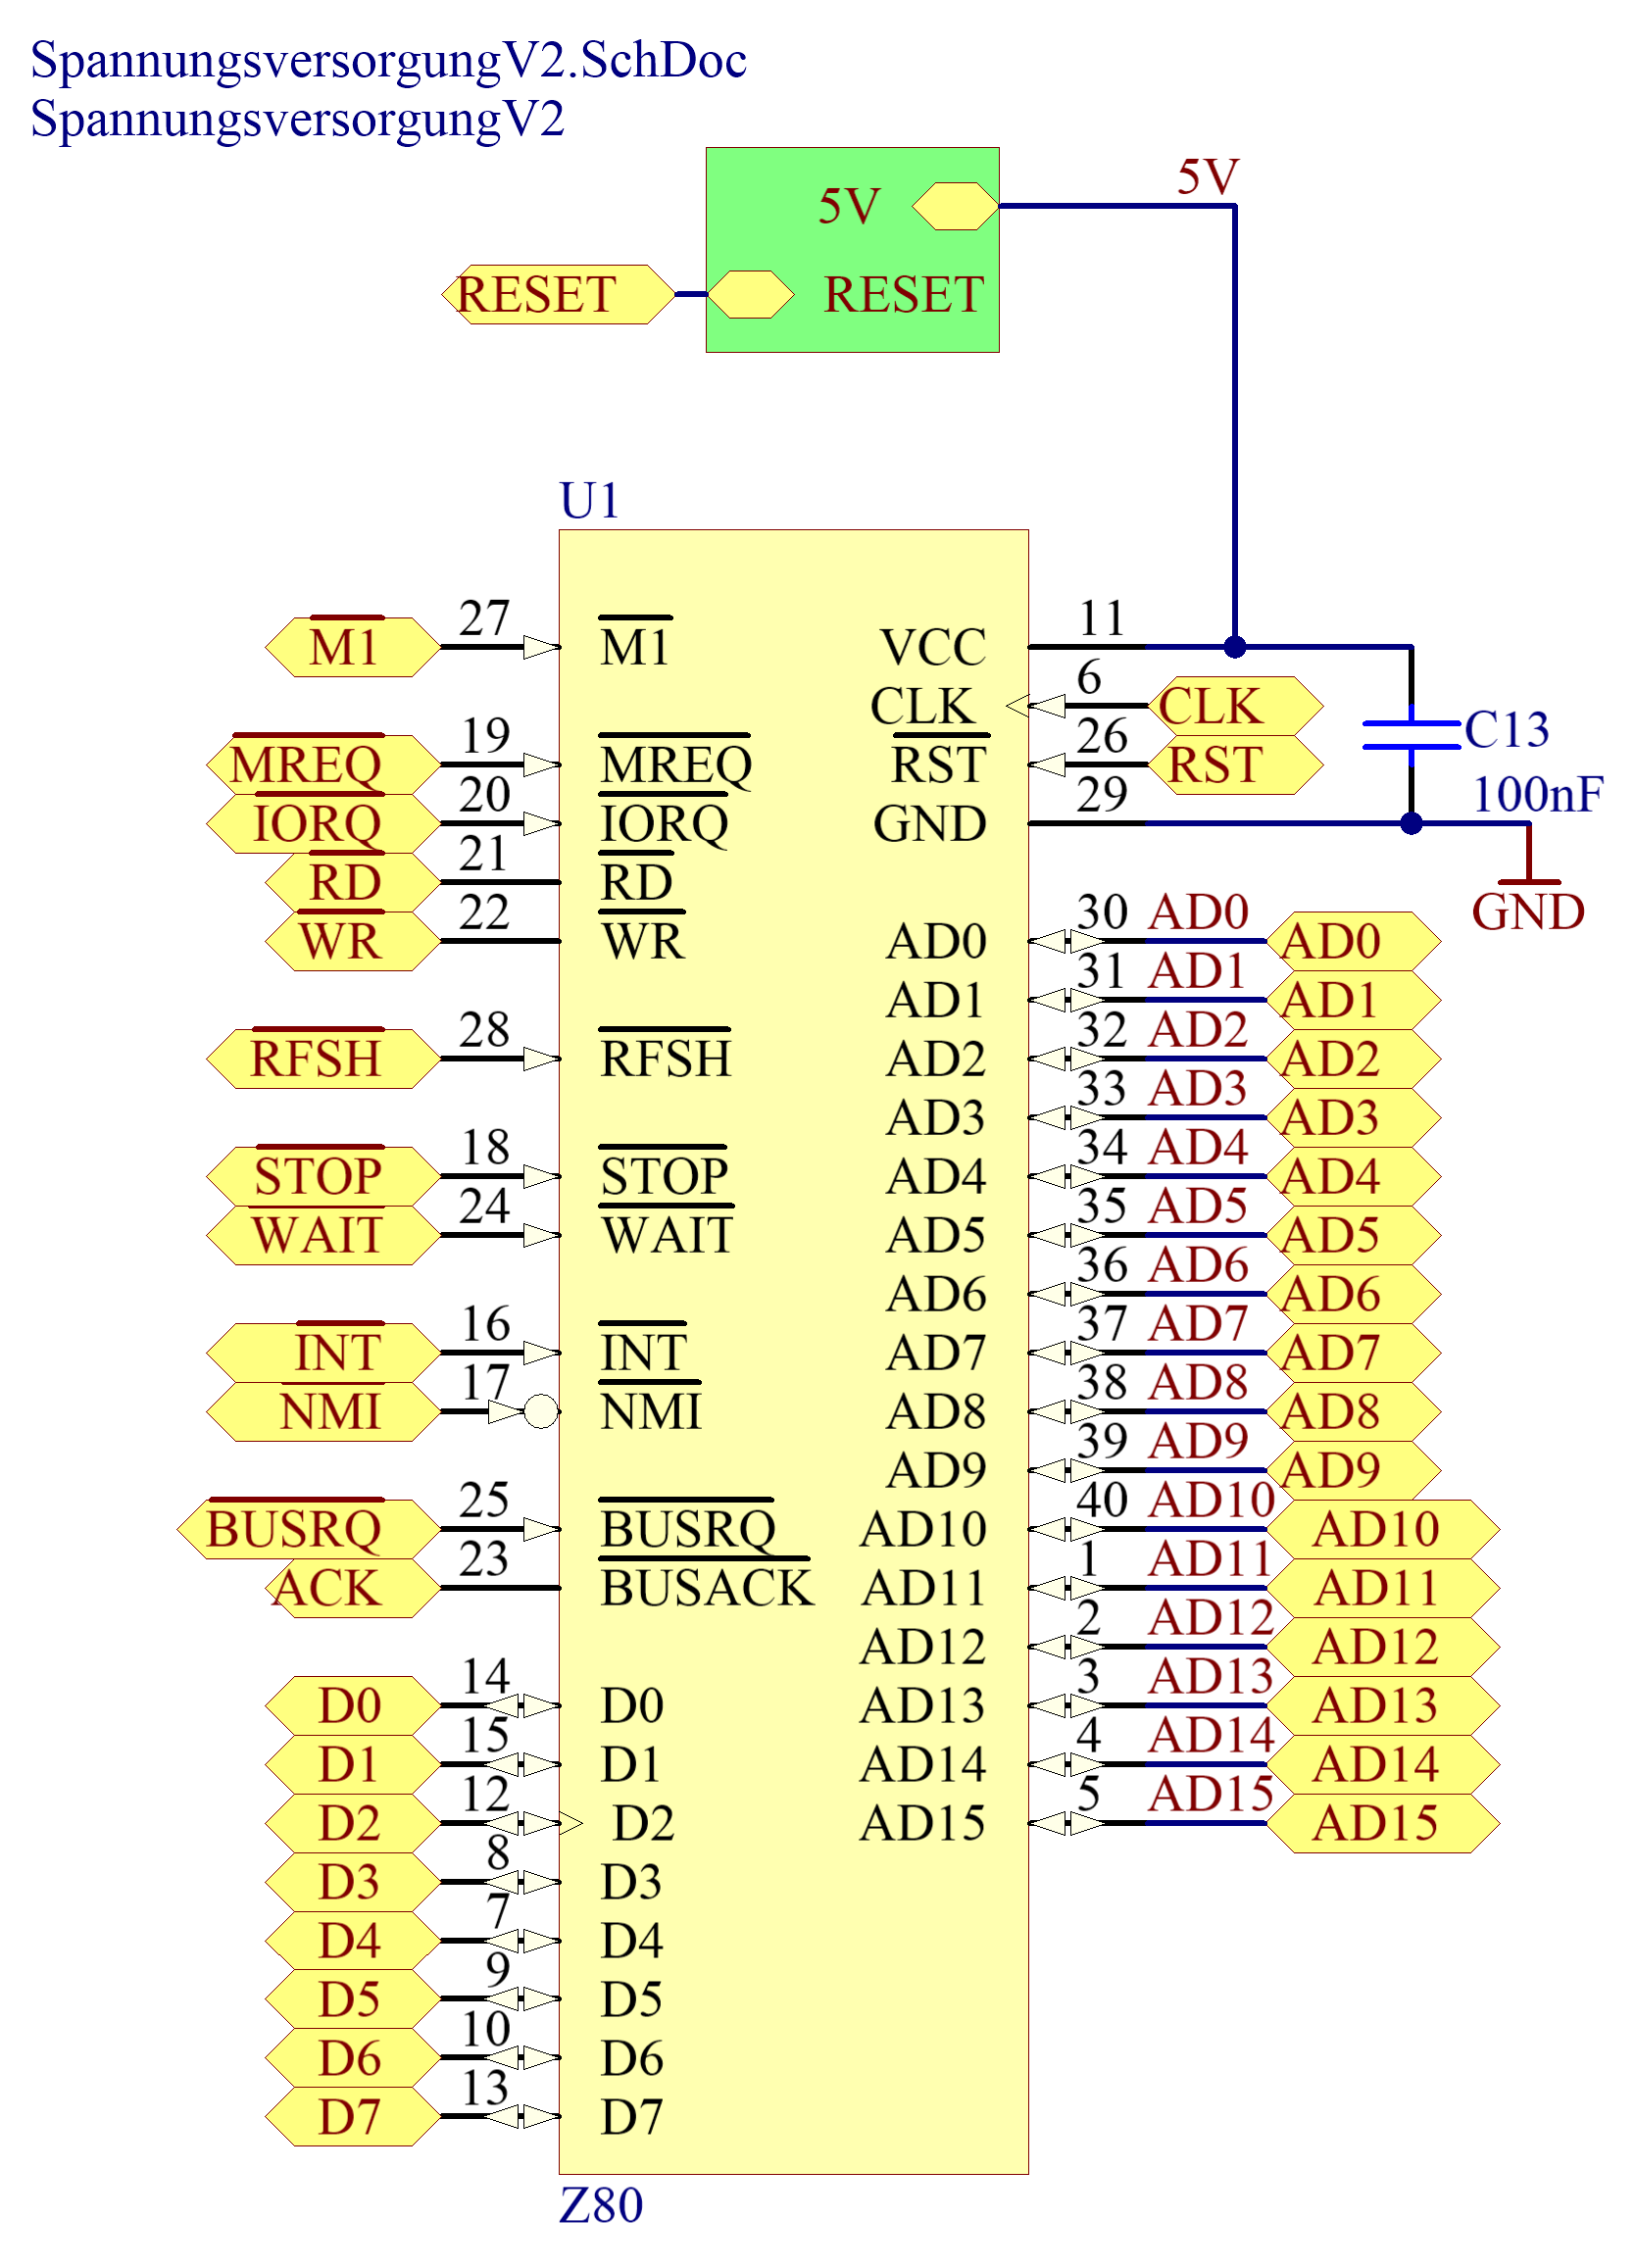
\includegraphics[width=.4\linewidth]{Reischl/img/z80-io-1}}\qquad
    \subfloat{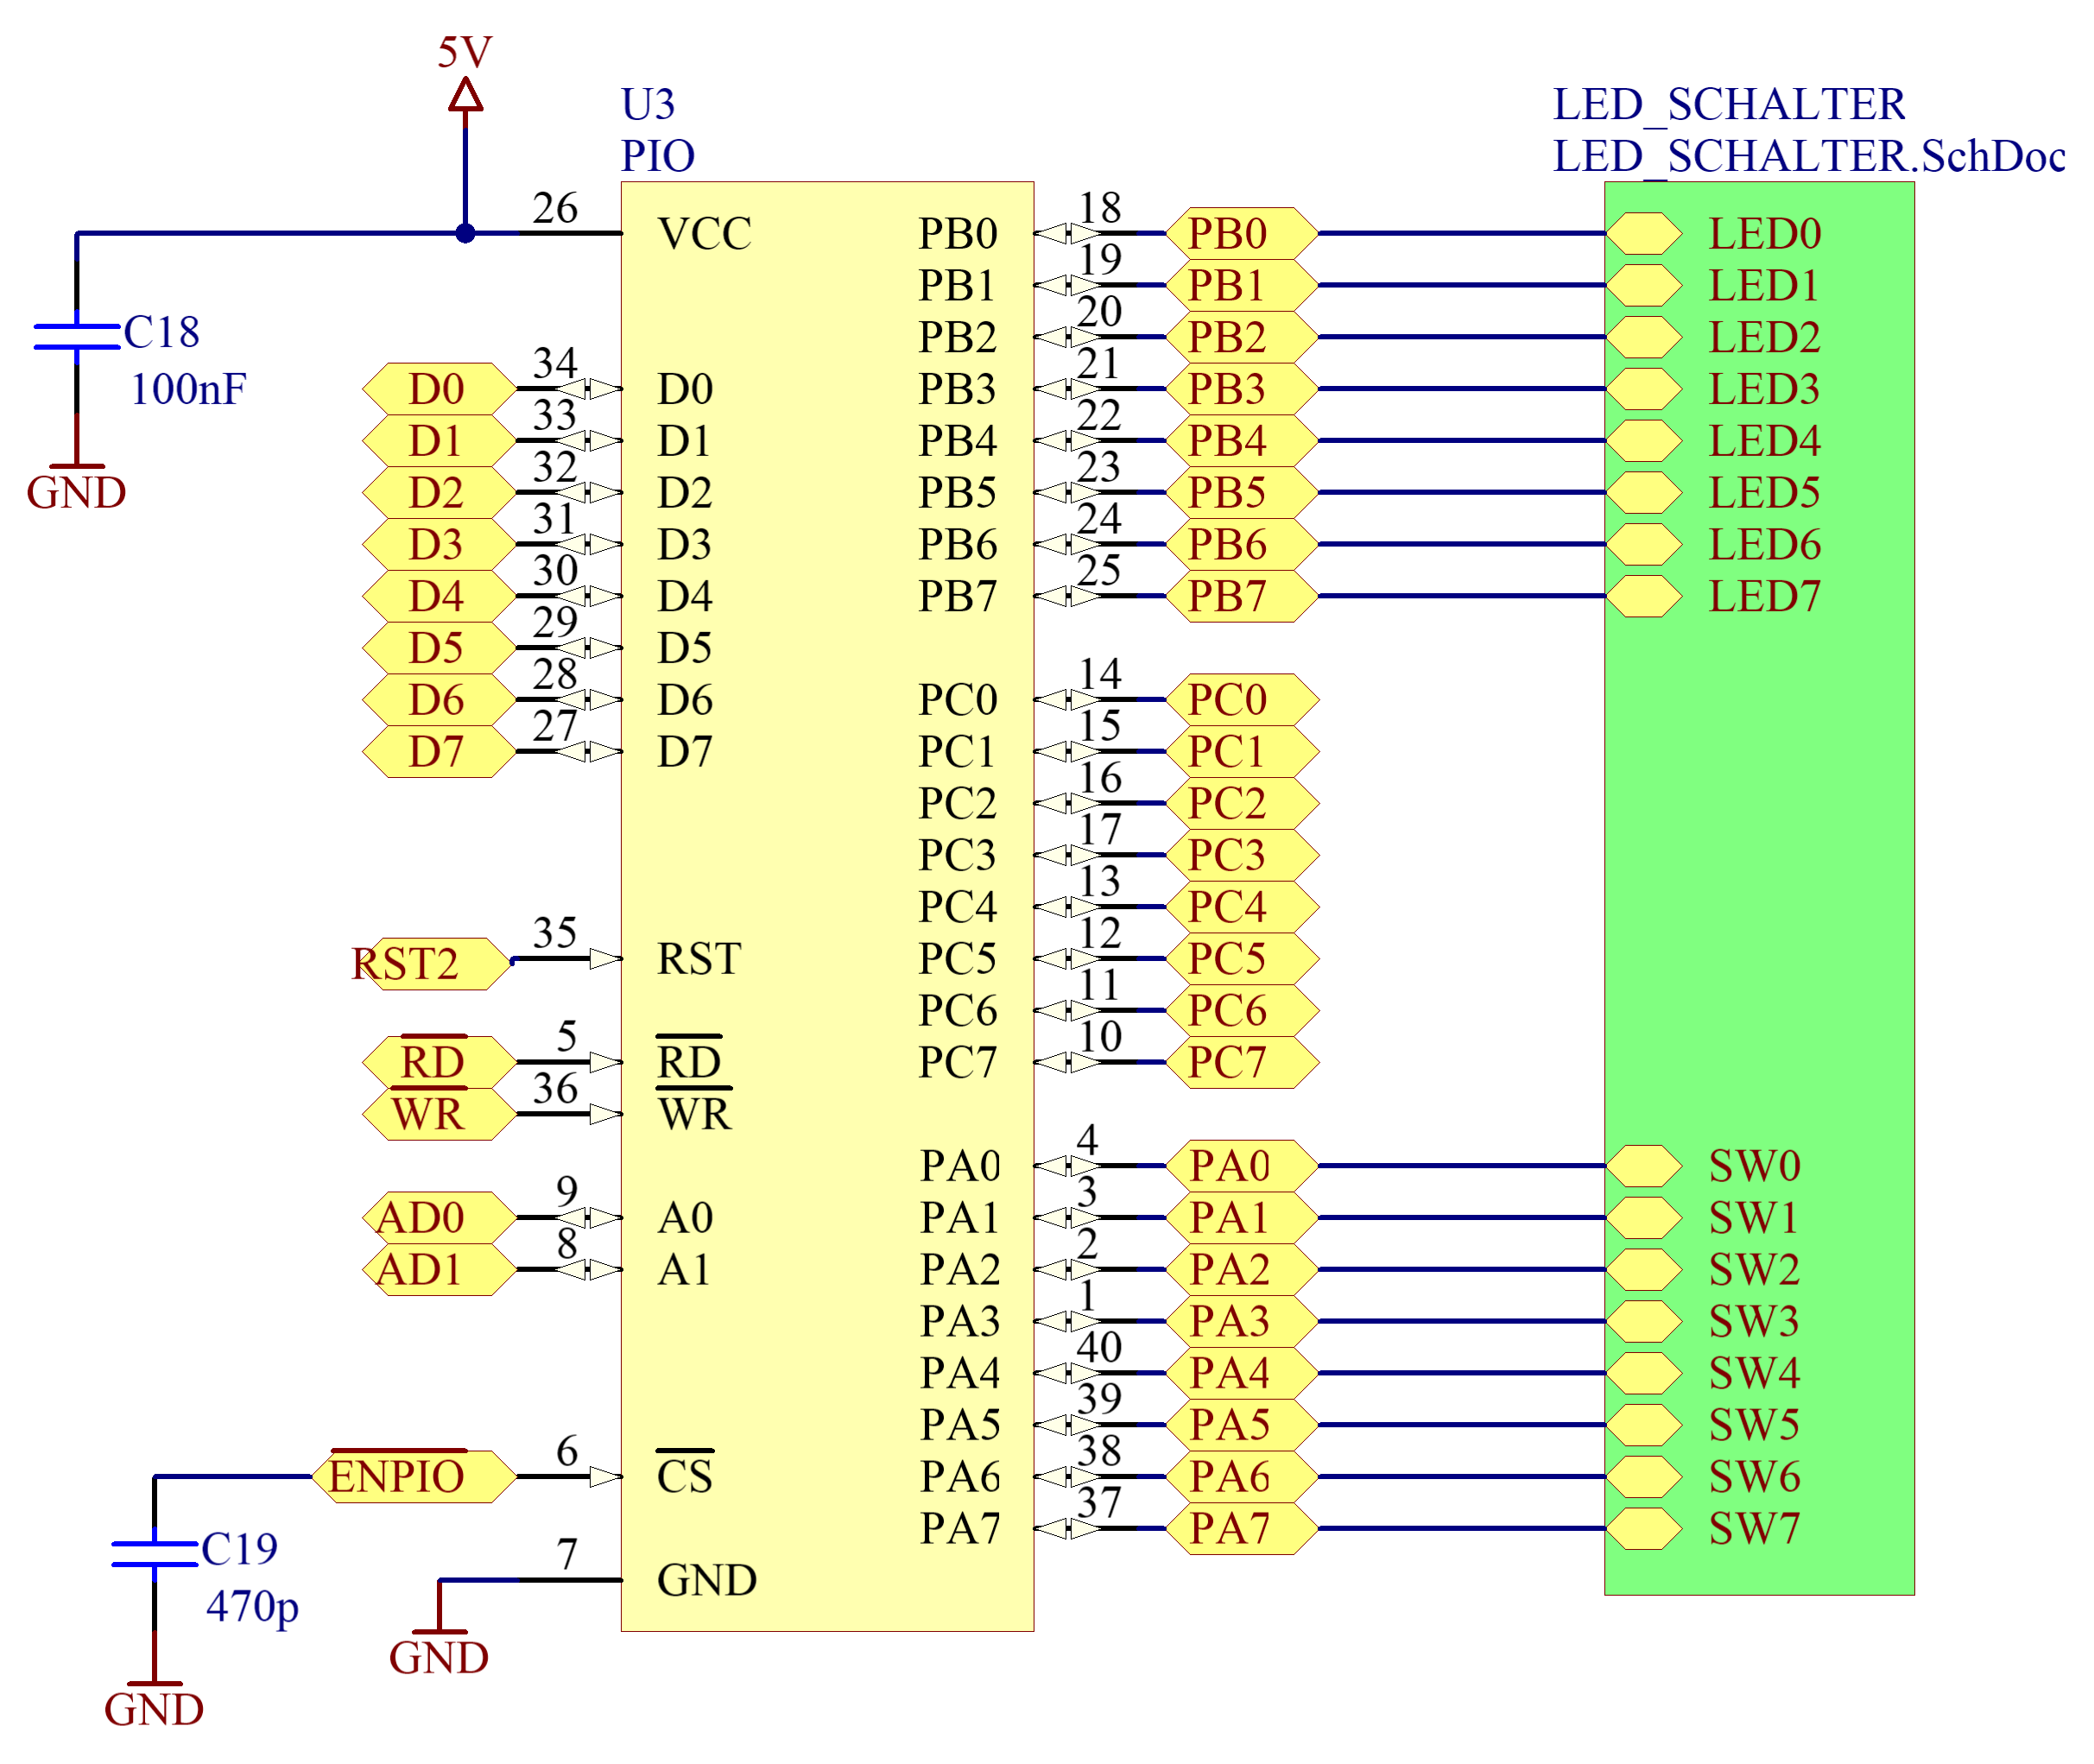
\includegraphics[width=.4\linewidth]{Reischl/img/z80-io-2}}\qquad
    \subfloat{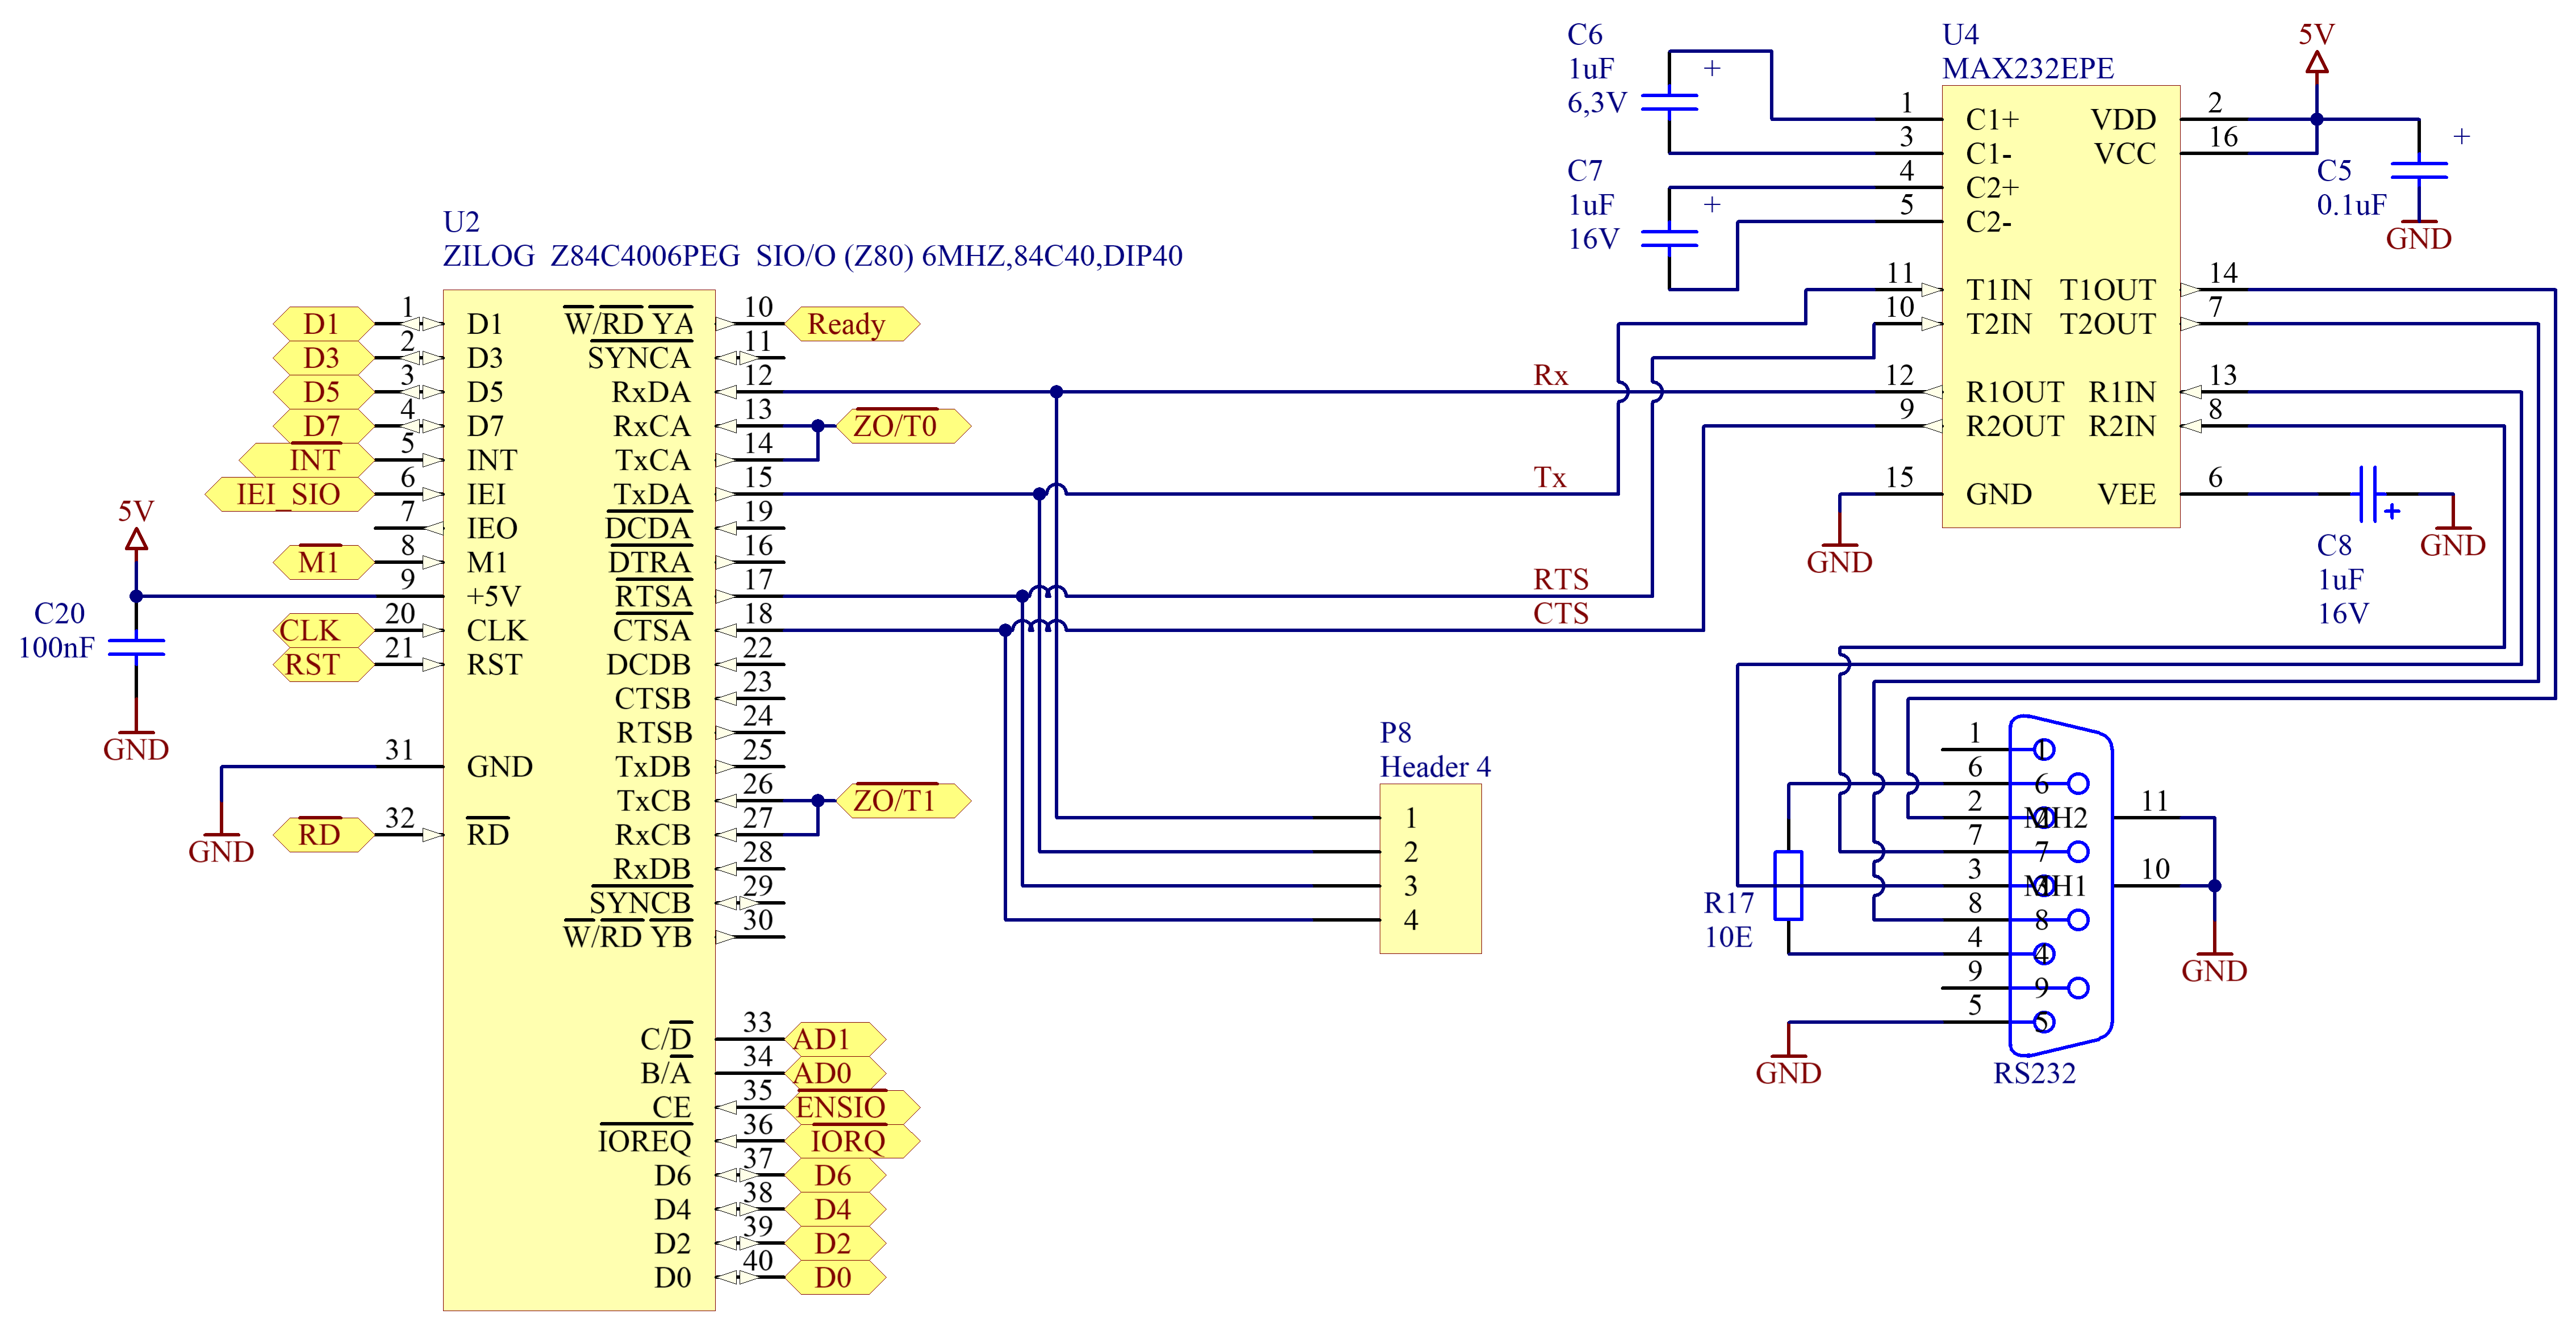
\includegraphics[width=\linewidth]{Reischl/img/z80-io-3}}\qquad
    \caption[Z80 Ein-/Ausgabeeinheiten]{Ein- und Ausgabeeinheiten}
    \label{fig:z80-io}
\end{figure}
Für den Informationsaustausch des Minimalsystems mit anderen Geräten oder mit dem Anwender besitzt die CPU einen 8-fach DIL-Schalter für das Einlesen von Daten, ein 8-fach LED-Array für die Ausgabe von Daten und eine serielle Schnittstelle, genau genommen eine RS233-Schnittstelle, für den Datenaustausch etwa mit einem Terminal.

Für Konfiguration und Datenaustausch mit der CPU nutzt der PIO und der SIO den gesamten 8 Bit breiten Datenbus und die ersten 2 Bit (AD0 und AD1) des 16 Bit breiten Adressbusses. Der Ablauf des Datenaustausches wird beim PIO neben dem Enable über die Signale Read und Write gesteuert. Dafür wird ein Port adressiert, der PIO enabled und mit dem Read oder Write angezeigt, ob gelesen oder geschrieben werden soll.

Der SIO nutzt den Datenbus dafür, um zu übermitteln, welcher Port (AD0: 0=A; 1=B) angesprochen wird und ob konfiguriert wird (AD1=1) oder ob Daten übertragen werden (AD1=0). Der IEI-Eingang ist Teil der Daisy Chain zur Priorisierung von Interrupts, da auch der DMA Controller und der CTC Interrupts auslösen kann. Die als Ready bezeichnete Leitung wird verwendet, um dem DMA-Controller den Status der Datenübertragung mitzuteilen. Mittels RD (Read) und IOREQ (I/O Request) wird die Datenübertragung von der CPU gesteuert, das SIO Enable aktiviert den SIO bzw. die Daten- und Adressleitungen. M1, also die Leitung, welche einen Machine Cycle One, also einen Instruction Fetch kennzeichnet, bewirkt gemeinsam diese gemeinsam mit einem I/O Request einen Interrupt, wenn über die Daisy Chain (IEI) der SIO die höchste Priorität erhält.

\subsection{Steuer zeitabhängiger Vorgänge}
\begin{figure}[htb]
    \centering
    \subfloat{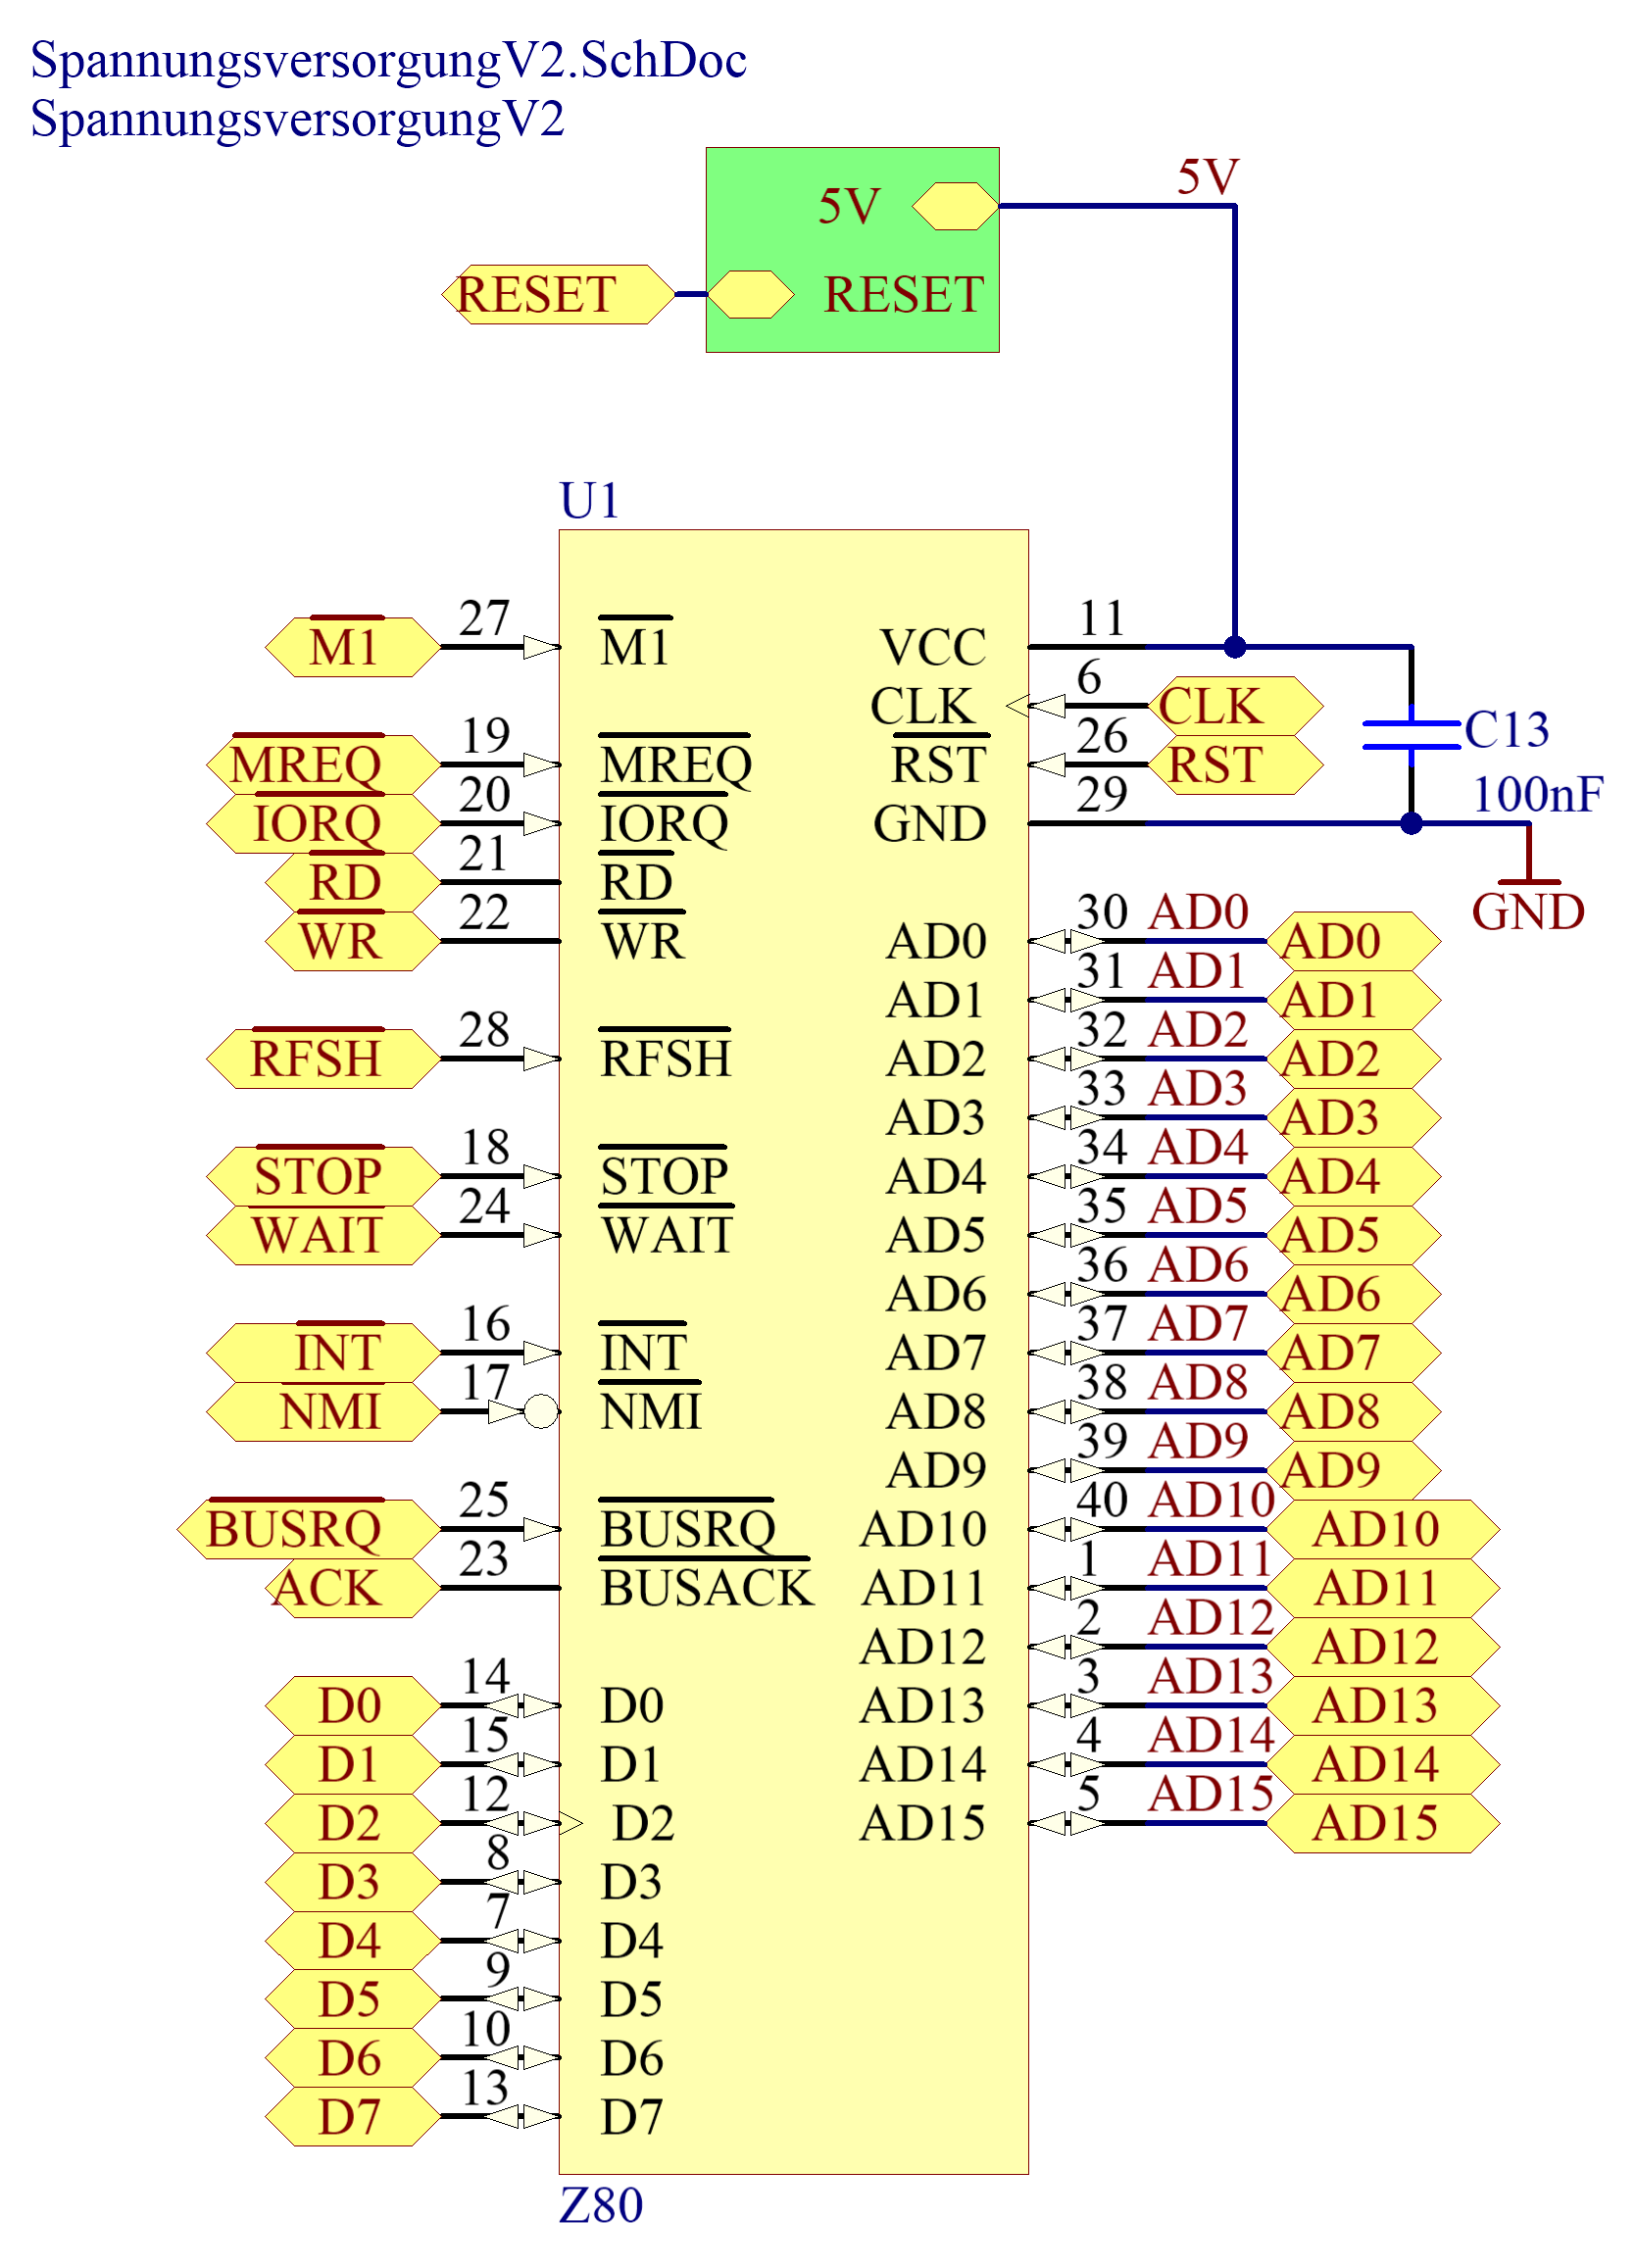
\includegraphics[width=.4\linewidth]{Reischl/img/z80-zeit-1}}\qquad
    \subfloat{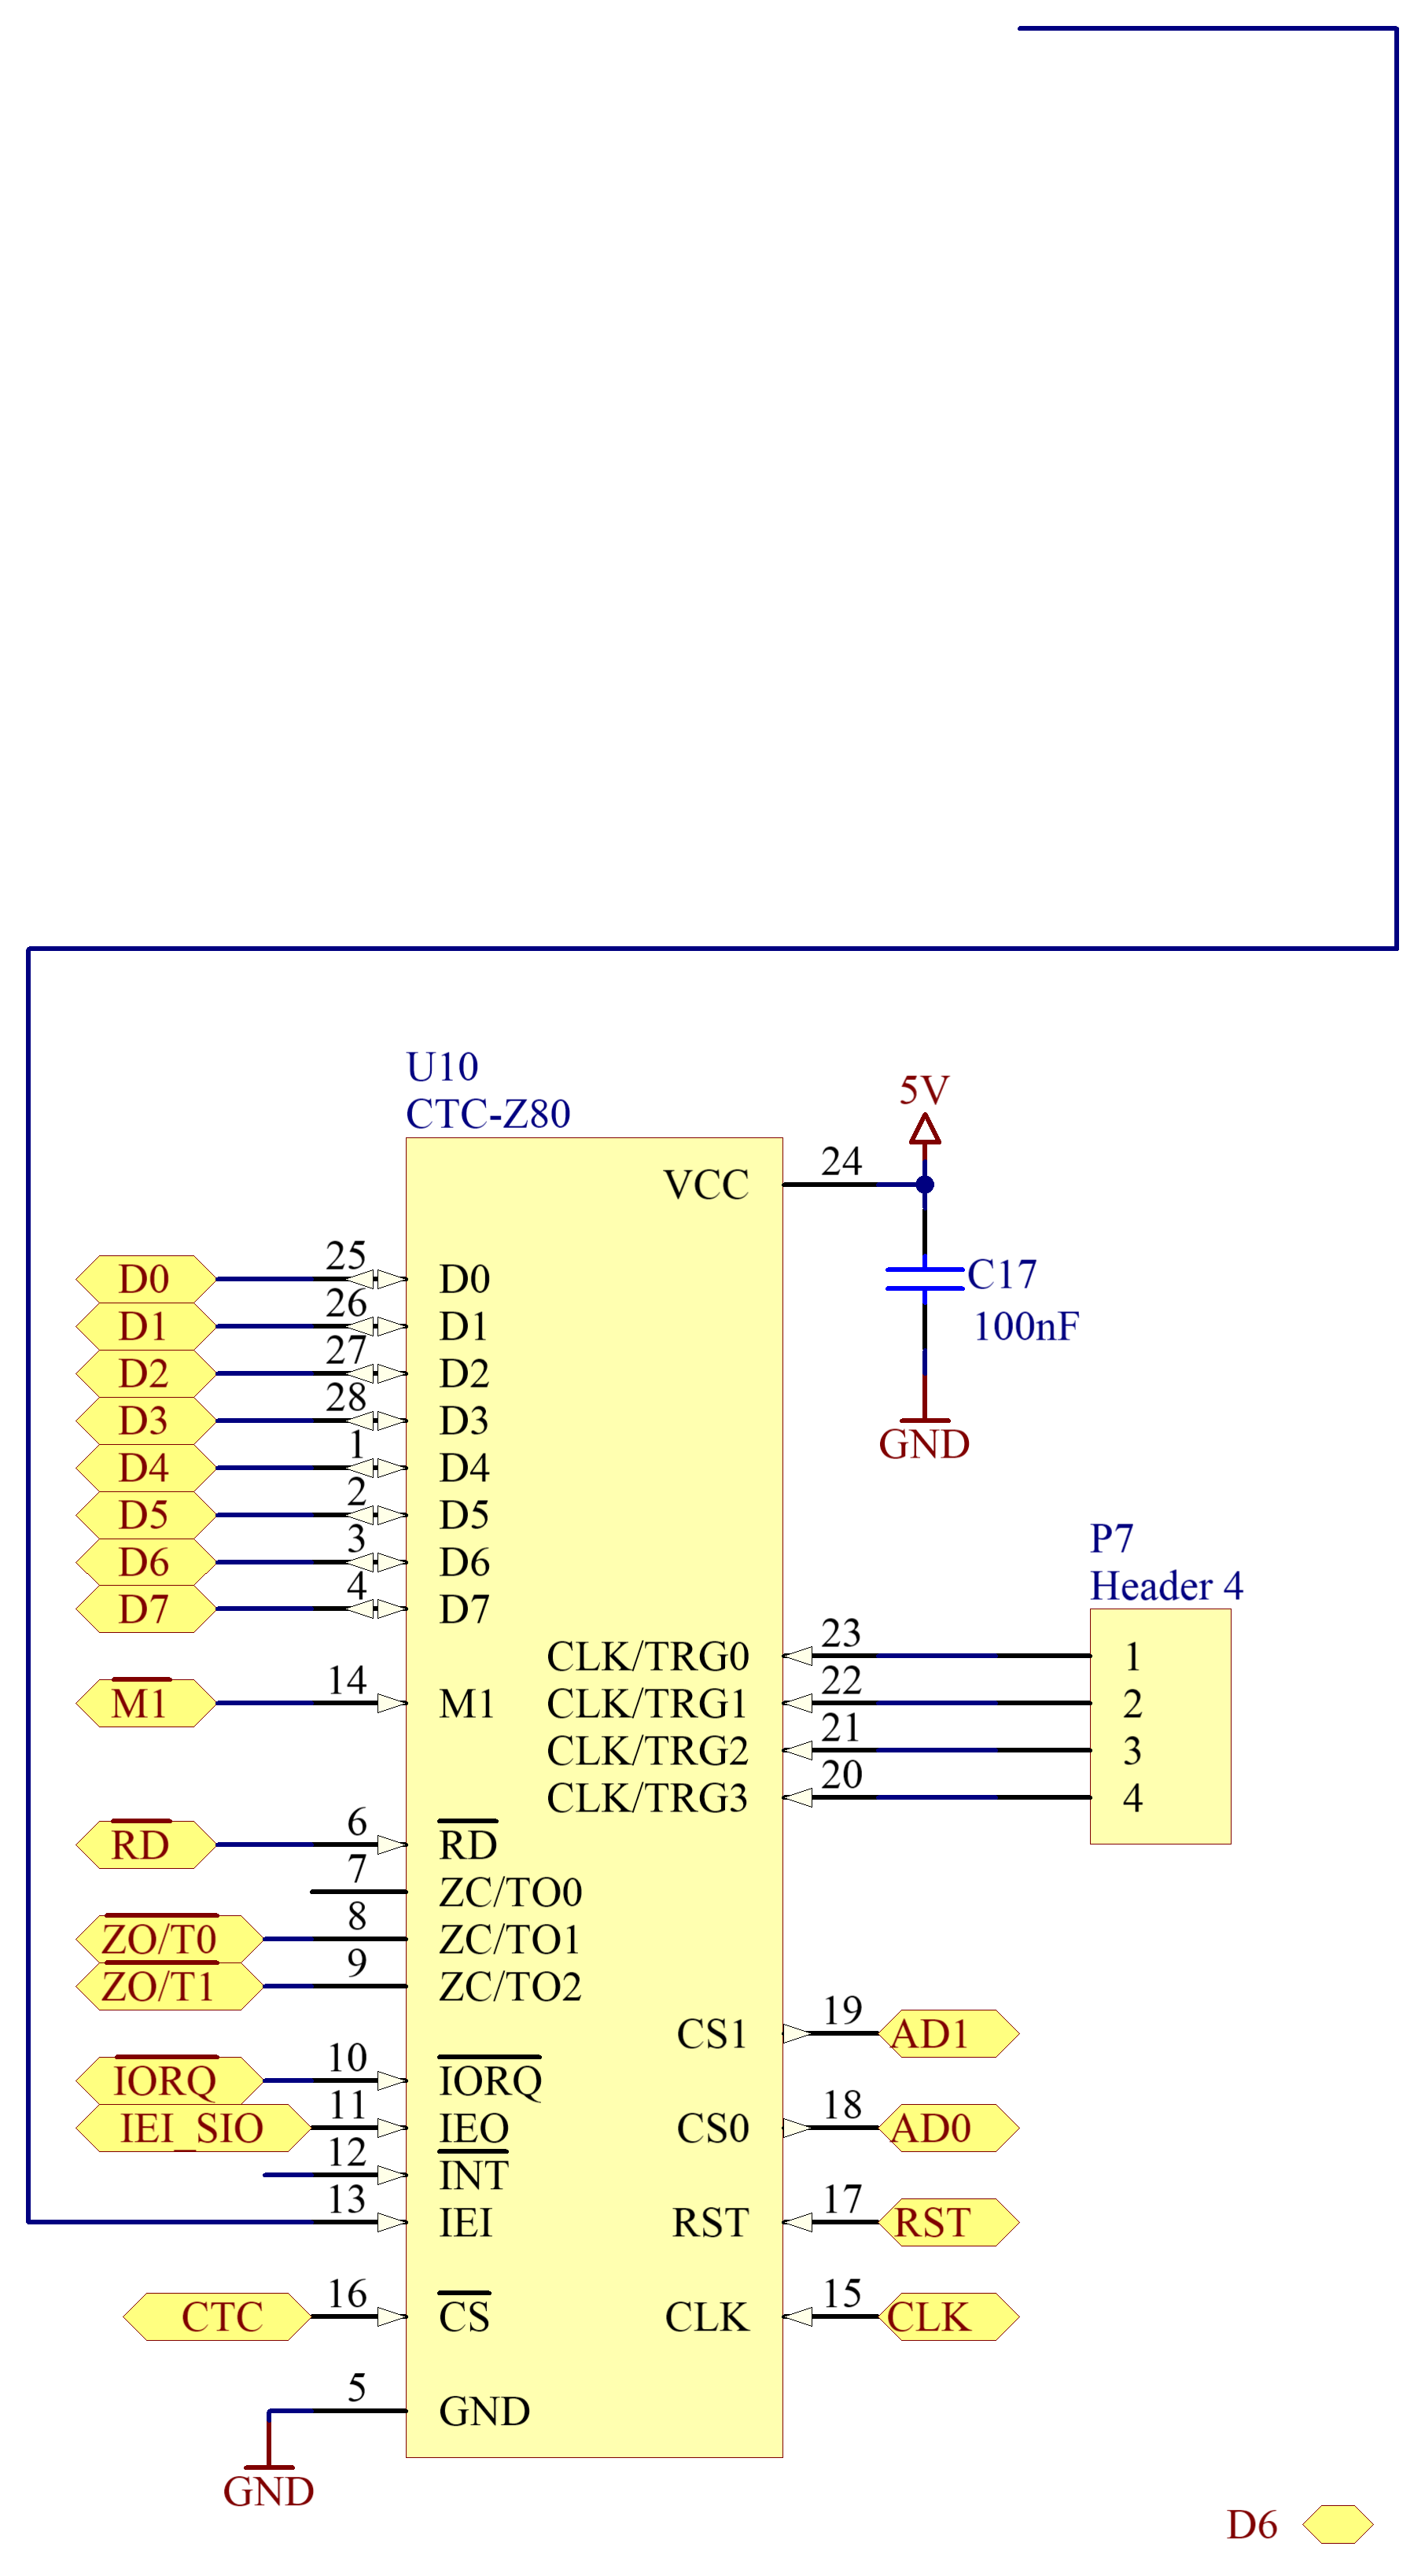
\includegraphics[width=.4\linewidth]{Reischl/img/z80-zeit-2}}\qquad
    \caption[Z80 Zeitabhängige Vorgänge]{Zeitabhängige Vorgänge}
    \label{fig:z80-zeit}
\end{figure}
Da der Counter-Timer-Circuit wie im nächsten Kapitel beschrieben sowohl als Timer als auch als Zähler eingesetzt werden kann, besitzt jeder Kanal einen Eingang CKT/TRGx, welcher als Eingang für den Zähler oder Start für den Timer genutzt werden kann. Der Daten- und Adressbus mit den Steuersignalen IO Request, Read und CS bzw. CTC dienen vor allem der Konfiguration, die Funktionen von M1 und IEI entsprechen den Erläuterungen zum SIO. Für genauere Informationen ist entweder das Datenblatt des verwendeten Bausteins oder das \textit{Z80 Family CPU Peripherals User Manual \cite{z80:periph}} heranzuziehen.

\subsection{Speicherzugriff durch die Peripherie}
\begin{figure}[htb]
    \centering
    \subfloat{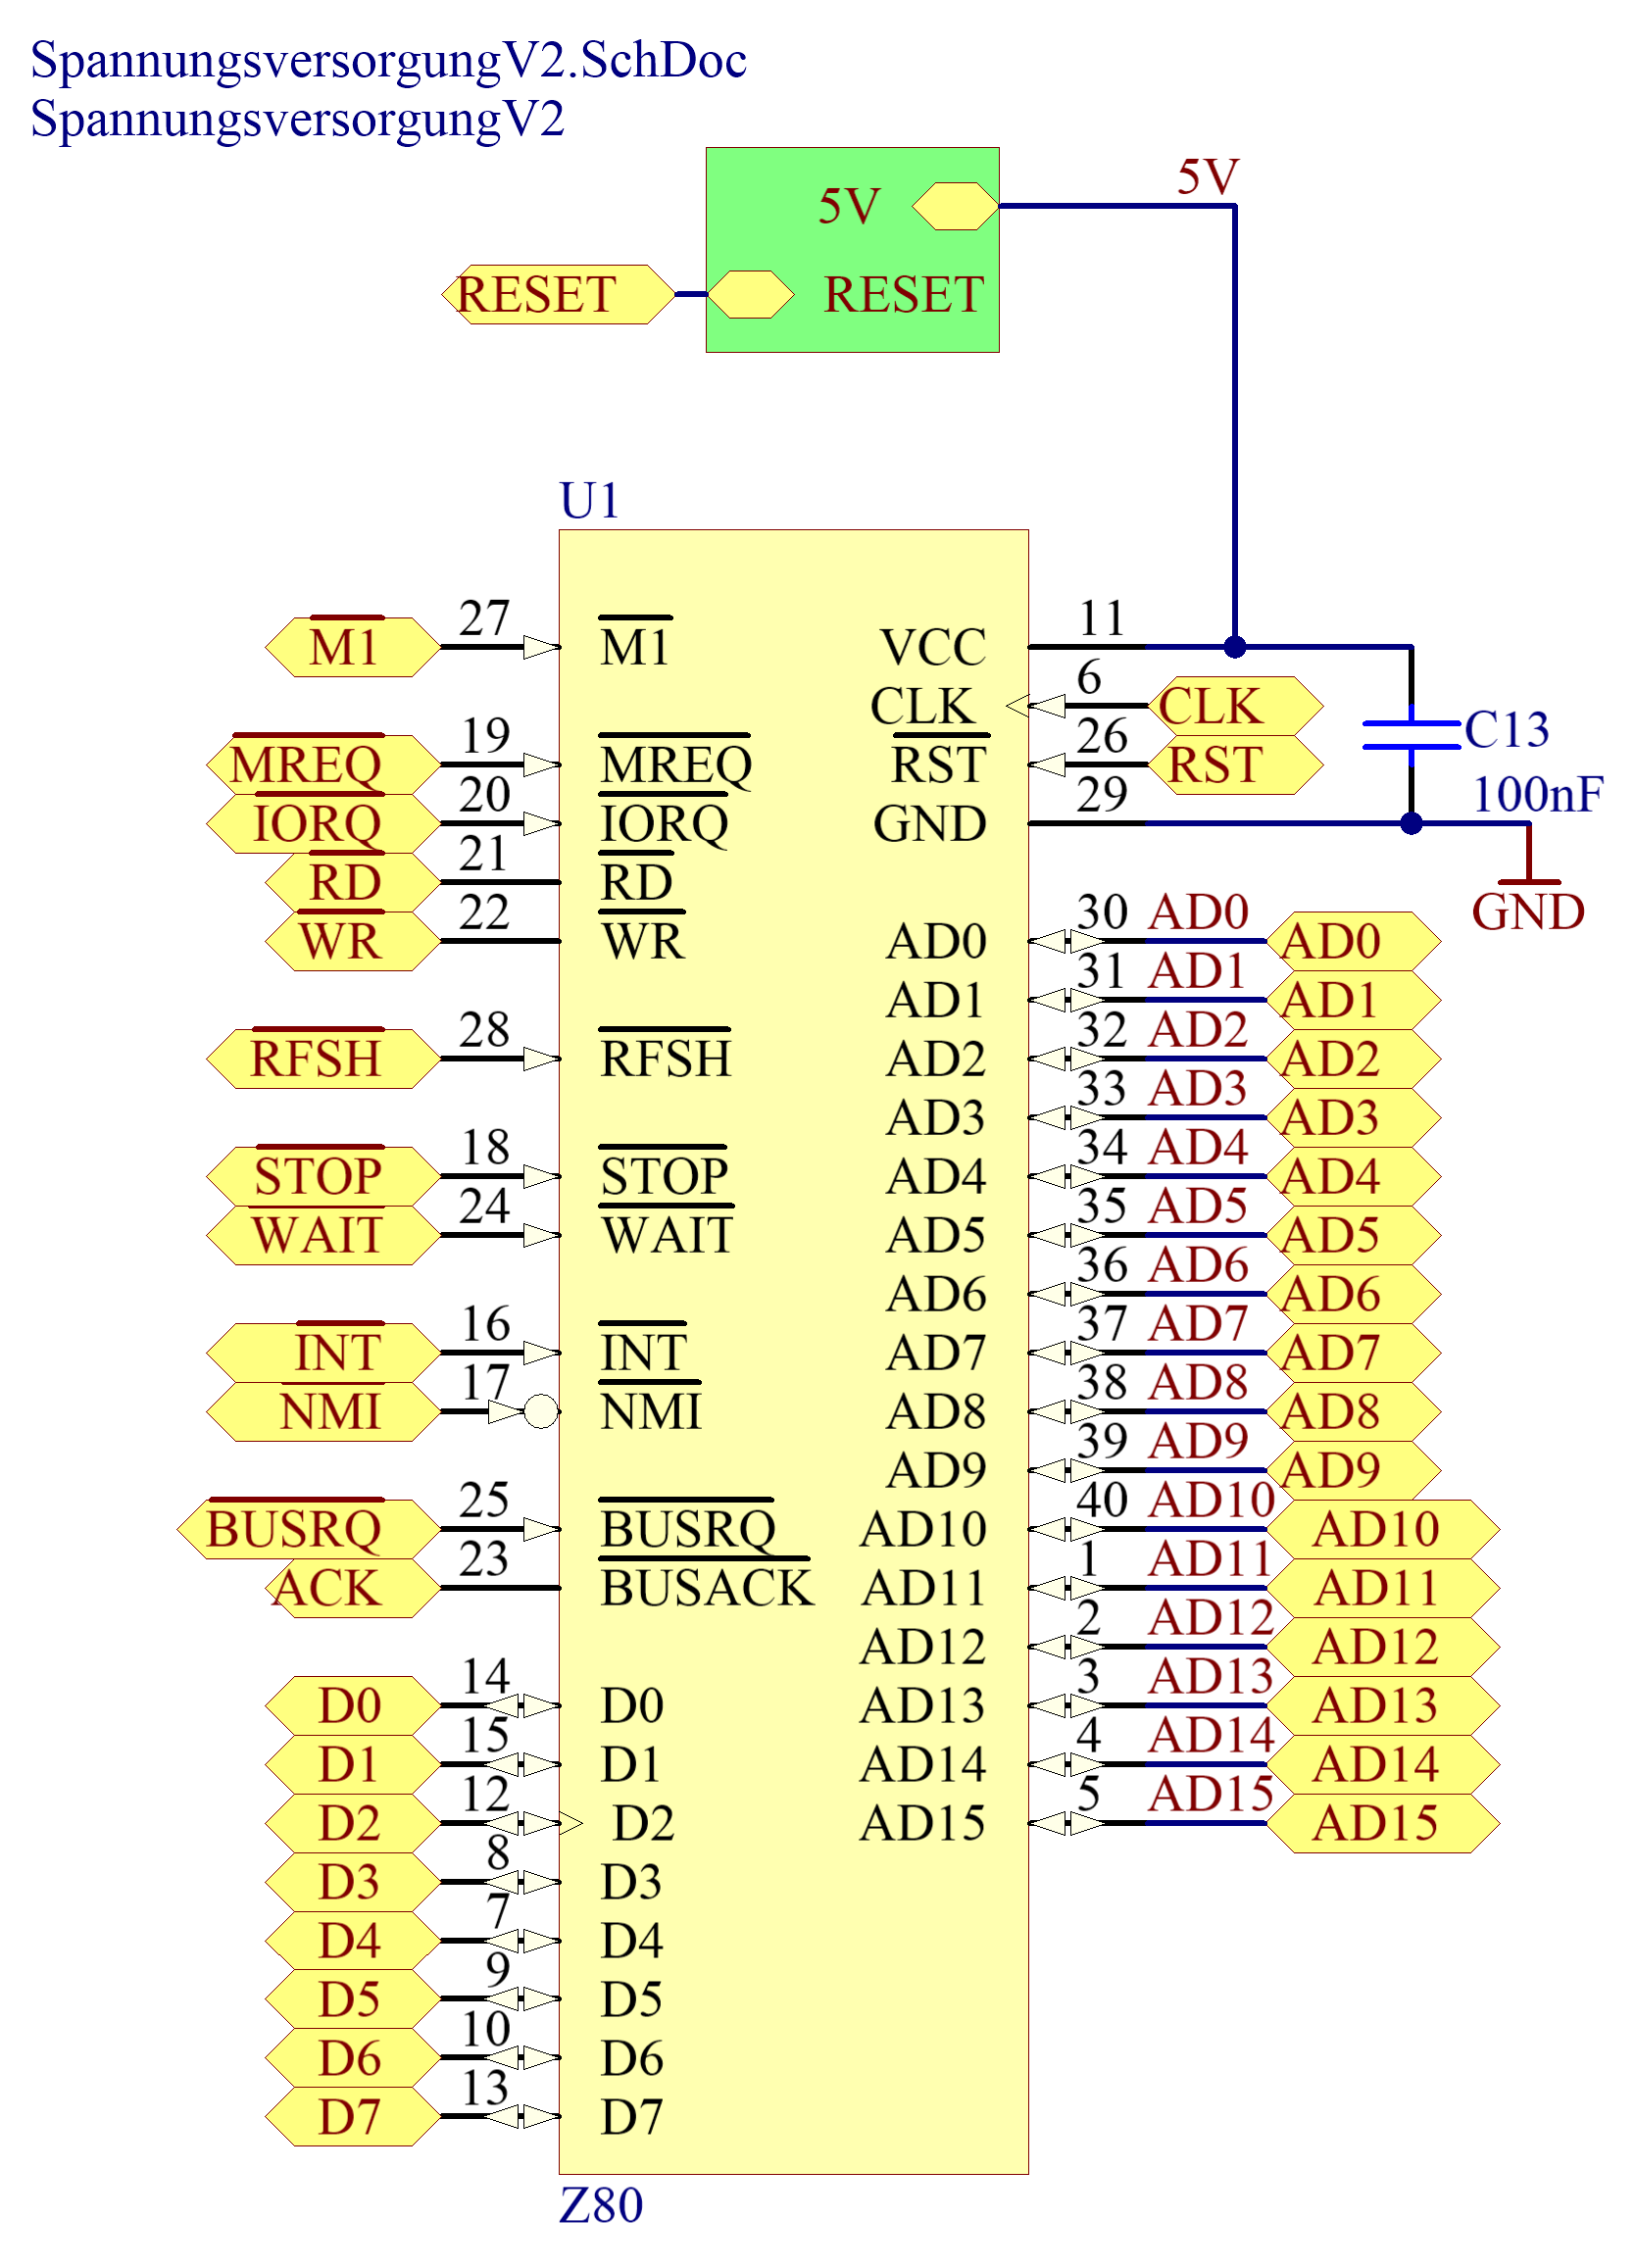
\includegraphics[width=.4\linewidth]{Reischl/img/z80-speicherper-1}}\qquad
    \subfloat{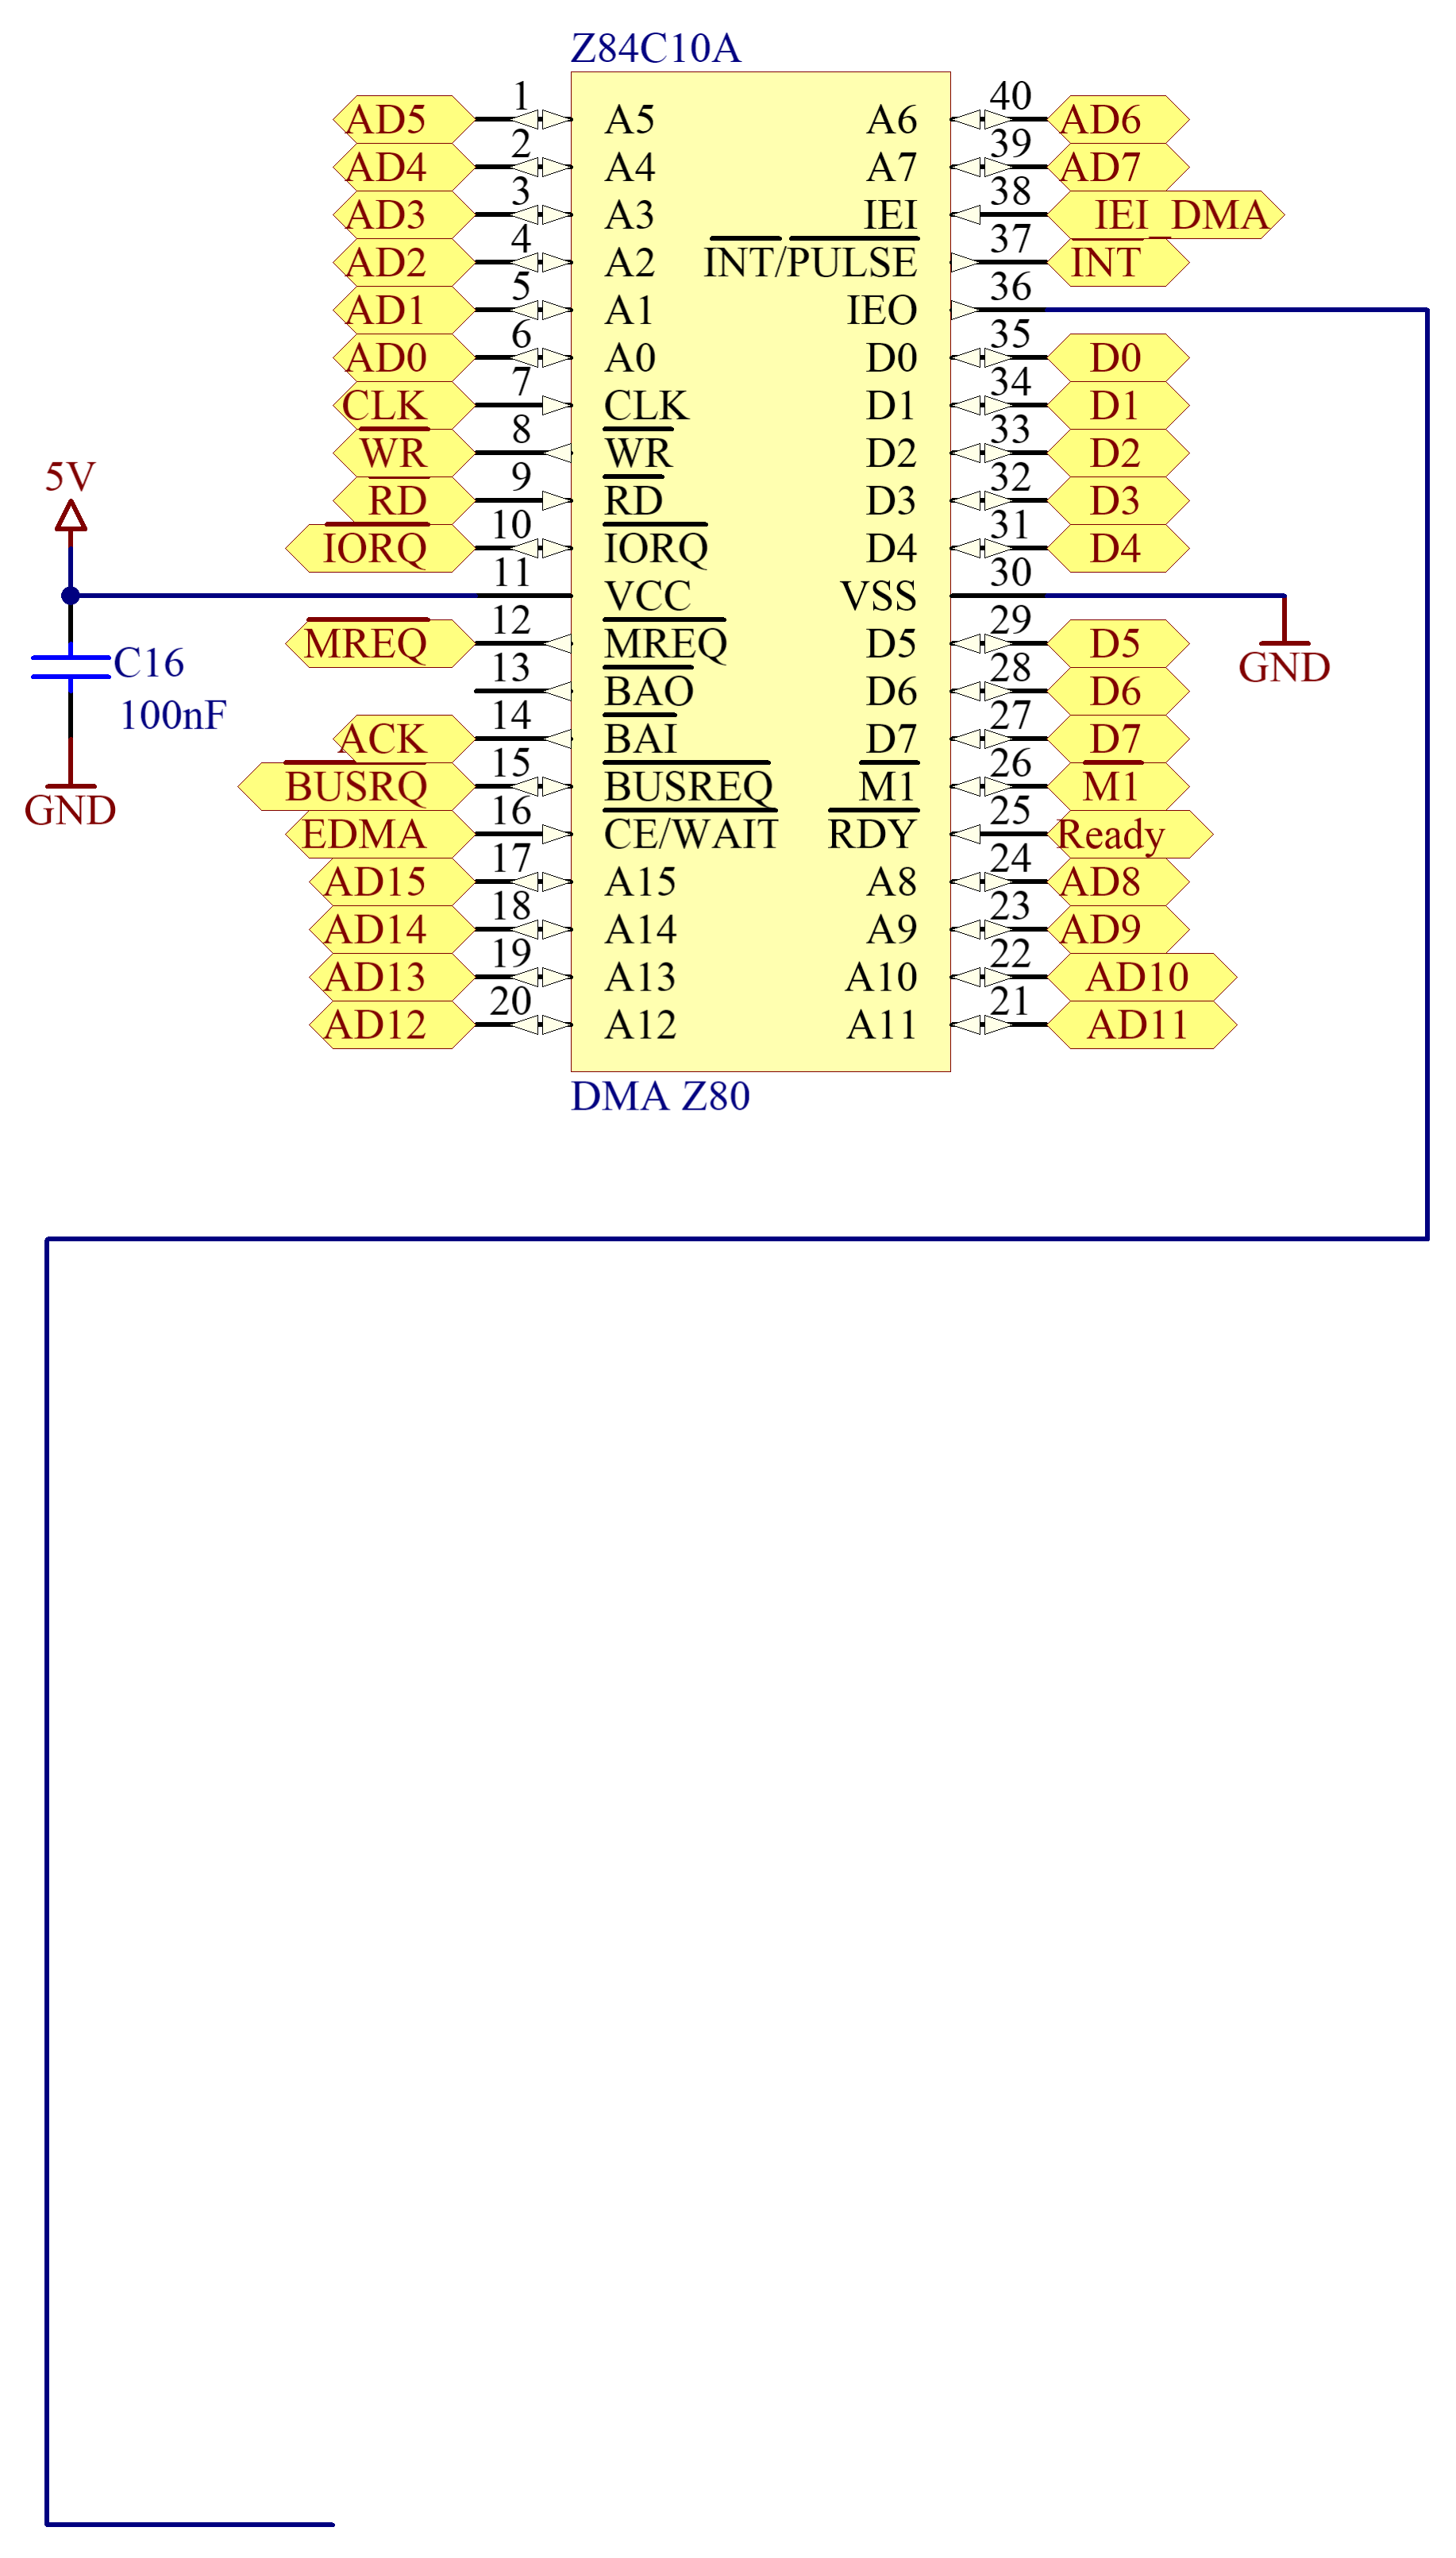
\includegraphics[width=.4\linewidth]{Reischl/img/z80-speicherper-2}}\qquad
    \caption[Z80 Speicherdirektzugriff]{Speicherdirektzugriff}
    \label{fig:z80-zeit}
\end{figure}
Der DMA Controller ermöglicht Speicherdirektzugriffe und Abarbeitung von Daten mit einer $2^n$ fachen Frequenz des Systemtaktes. Der DMAC besitzt wie der SIO und der CTC die Möglichkeit, einen Interrupt (INT) auszulösen und ist somit Teil der Daisy Chain (IEI). Bei einer Datenübertragung, die nicht von der CPU selbst vorgenommen wird, ist es wichtig, darauf zu achten, dass der Daten- und Adressbus nicht gleichzeitig von mehreren Baugruppen verwendet wird. Dies wird durch das Acknowledge (BAI bzw. ACK) überprüft, über den Busrequest (BUSREQ) wird der Übertragungsvorgang gesteuert. I/O Request, Memory Request, Read und Write dienen der Steuerung des Speicher- bzw. Peripheriezugriffs, die Funktion von IEI ist der Beschreibung des SIO zu entnehmen. Detailliertere Informationen sind im Z80 Family CPU Peripherals User Manual \cite{z80:periph} zu finden.

\subsection{Gesamtschaltung}
\fig{z80-pcb}{Z80 PCB}{PCB}{\textwidth}{Reischl/img/z80-pcb}
\begin{figure}[htb]
    \centering
    \subfloat[Mainsheet 1]{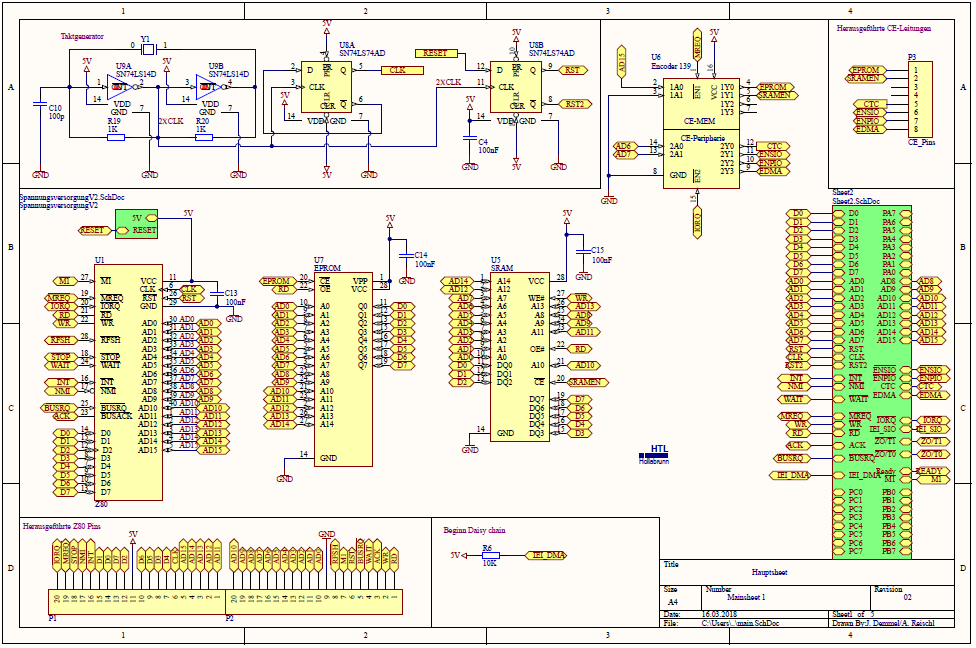
\includegraphics[width=\linewidth]{Reischl/img/z80-gesamt-1}}\qquad
    \subfloat[Mainsheet 2]{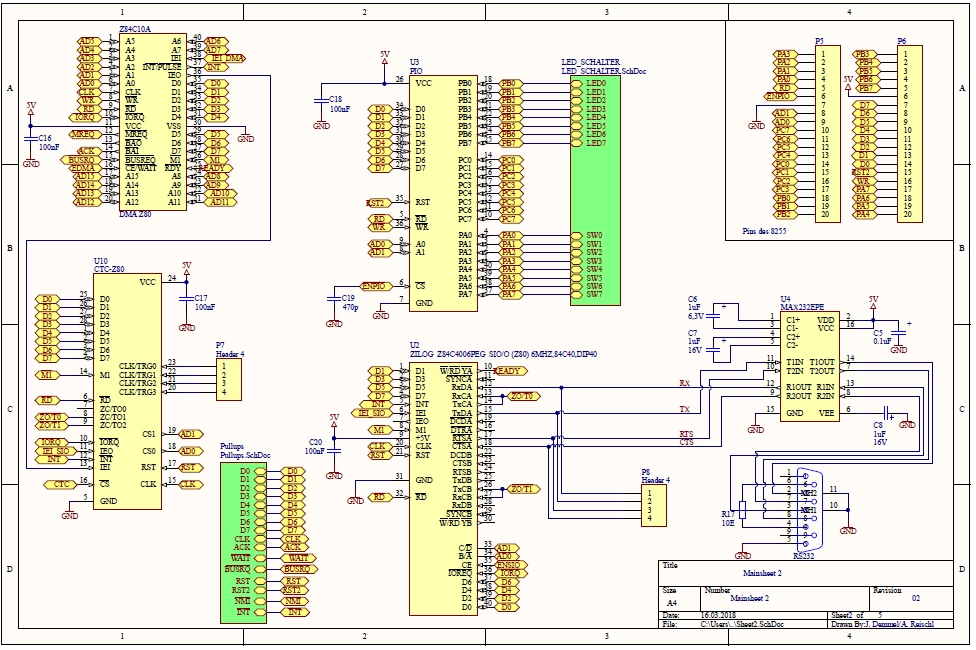
\includegraphics[width=\linewidth]{Reischl/img/z80-gesamt-2}}\qquad
\end{figure}
\begin{figure}[htb]
    \ContinuedFloat
    \subfloat[Spannungsversorgung]{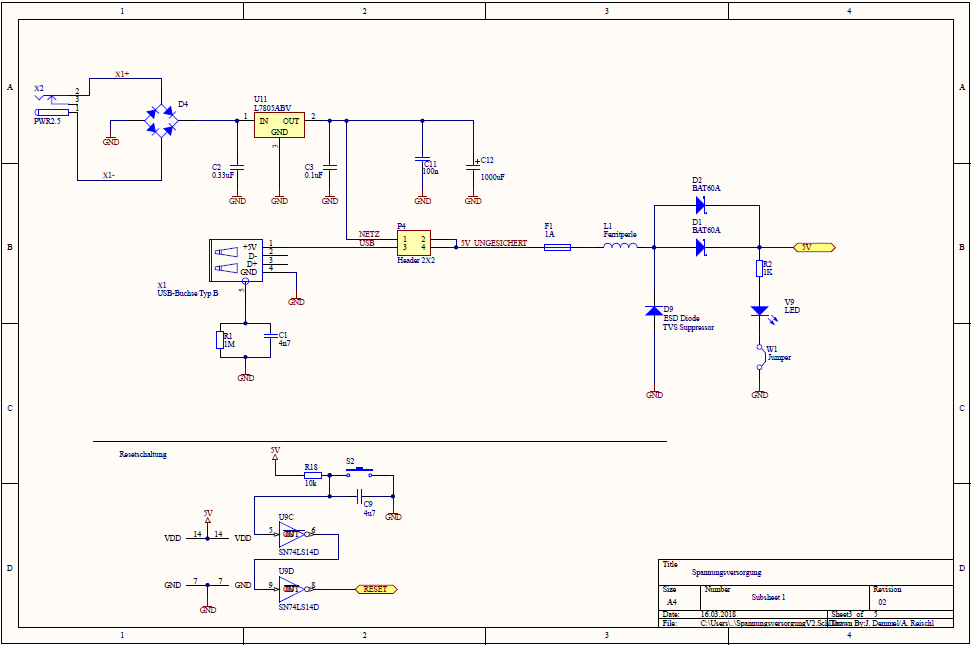
\includegraphics[width=\linewidth]{Reischl/img/z80-gesamt-3}}\qquad
    \subfloat[LED und Schalter (I/O)]{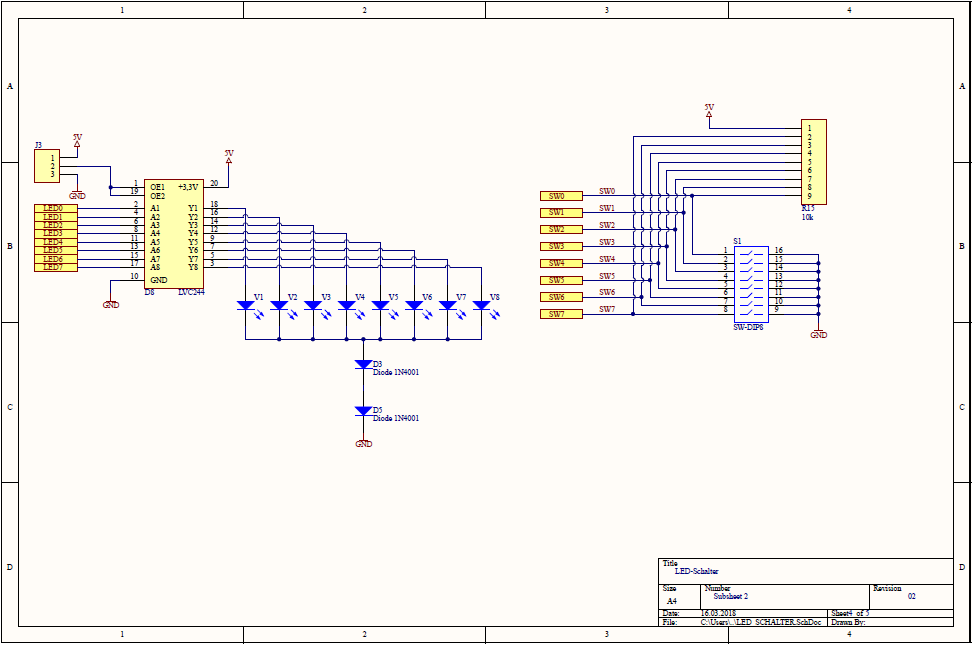
\includegraphics[width=\linewidth]{Reischl/img/z80-gesamt-4}}\qquad
\end{figure}
\begin{figure}[htb]
    \ContinuedFloat
    \subfloat[Pull-Ups]{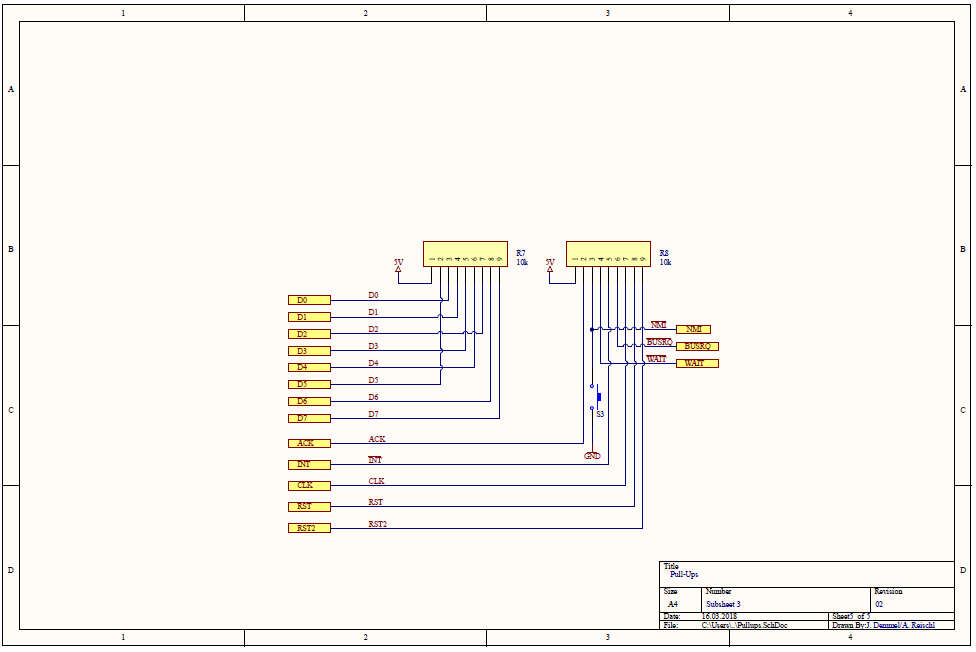
\includegraphics[width=\linewidth]{Reischl/img/z80-gesamt-5}}\qquad
    \caption[Z80 Schematics]{Schematics}
    \label{fig:z80-zeit}
\end{figure}

\section{Baugruppen des Z80 Minimalsystems}
\label{sec:z80-baugruppen}
\subsection{Spannungsversorgung}
Die gesamte Hardware, die beim Z80 Minimalsystem zum Einsatz kommt, benötigt eine Betriebsspannung von 5V Gleichspannung, die erlaubte Schwankungsbreite der Spannung liegt bei allen systemspezifischen Komponenten und bei den verwendeten Logikgattern laut den einzelnen Datenblättern in einem Bereich von 4,75V bis 5,25V. Die Anforderung an die Spannungsversorgung war neben der guten Verfügbarkeit der einzelnen Versorgungsarten ein möglichst geringer Störungsanteil bei gleichzeitig einfacher Umsetzbarkeit. Deshalb fiel die Wahl auf 2 verschiedene Versorgungsmöglichkeiten: Die erste Möglichkeit ist die Versorgung mittels Netzteil mit Linearregler auf dem Minimalsystem, bei der zweiten Variante handelt es sich um eine USB-Versorgung, deren Schnittstelle im Gegensatz zu den vorherigen Versionen nicht als Micro-USB ausgeführt ist, sondern als USB Typ B. Dadurch wird eine bessere mechanische Stabilität der Steckverbindung ermöglicht, außerdem werden USB-B Kabel mit größeren Leitungsquerschnitten angeboten, wodurch der Spannungsabfall an der Versorgung so weit reduziert werden kann, dass die Untergrenze von 4,75V Betriebsspannung selbst bei der Verwendung von TTL Logik anstatt der aktuell verwendeten NMOS bzw. CMOS-Technologie eingehalten werden kann.

\subsubsection{Fixspannungsregler/Netzversorgung}
Bei dem verwendeten Fixspannungsregler vom Typ L7805CV handelt es sich um einen Linearregler des Herstellers ST Microelectronics. Dieser verfügt über eine Ausgangsspannung von 5V bei einem Maximalstrom von 1A. Die minimale Spannung am Ausgang liegt bei 4,8V, das Maximum beträgt 5,2V. Am Eingang dürfen abhängig vom Ausgangsstrom, der daraus resultierenden Verlustleistung und der Tatsache, ob und welcher Kühlkörper verwendet wird, bis zu 35V anliegen. Um einen störungsfreien Betrieb zu gewährleisten, ist der Linearregler entsprechend Datenblatt am Eingang mit einer Kapazität von 330nF und am Ausgang mit 100nF zu versehen.
\begin{figure}[htb]
    \subfloat[Gehäuse]{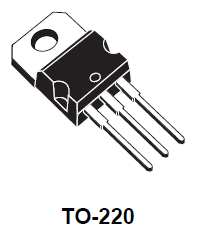
\includegraphics[width=.4\linewidth]{Reischl/img/z80-lin-1}}\qquad
    \subfloat[Pinning]{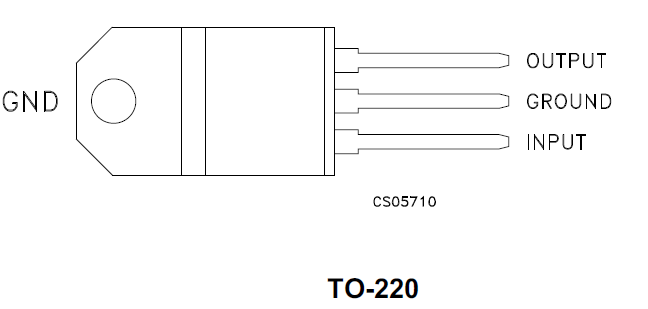
\includegraphics[width=.4\linewidth]{Reischl/img/z80-lin-2}}\qquad
    \caption[Z80 Linearregler Gehäuse und Pinning]{Linearregler Gehäuse und Pinning \cite{z80:lin}}
    \label{fig:z80-lin-1}
\end{figure}
\fig{z80-lin-2}{Z80 Linearregler Blockschaltbild}{L7805 Linearregler Blockschaltbild \cite{z80:lin}}{\textwidth}{Reischl/img/z80-lin-3}
Der am Minimalsystem verbaute Fixspannungsregler wurde am Eingang um einen Brückengleichrichter ergänzt, um einer Verpolung entgegenzuwirken und das System vor etwaigen Schäden durch den Betrieb mit einem AC-Netzteil zu schützen. Wenn möglich, sollte aber ein DC-Netzteil mit einer Ausgangsspannung 9V verwendet werden, um die Dropout Voltage nicht zu unterschreiten und gleichzeitig die Verlustleistung gering zu halten, da kein Kühlkörper verbaut wurde. Schnittstelle zwischen Minimalsystem und Netzteil bildet ein Niedervoltsteckverbinder, auch als PowerJack bezeichnet. Der verwendete Hohlstecker besitzt einen Außendurchmesser von 5,5 mm und einen Stift mit 2mm Durchmesser.
\fig{z80-lin-3}{Z80 Versorgung Netzteil}{Versorgung Netzteil \cite{z80:lin}}{\textwidth}{Reischl/img/z80-lin-4}

\subsubsection{USB Versorgung}
Das Minimalsystem verfügt über eine USB Typ B Buchse, um das Minimalsystem mithilfe des USB-Treibers eines Computers oder mit einem Ladegerät für Smartphones zu versorgen.
\fig{z80-usb}{Z80 Versorgung USB}{Versorgung USB}{0.3\textwidth}{Reischl/img/z80-usb}

\subsubsection{Wahl der Versorgungsart}
Das Umschalten zwischen USB- und Netzversorgung erfolgt mittels Jumper, der auf einer 2x2 poligen Stiftleiste umgesteckt wird. Wenn man Pin 1 und 2 verbindet, wird das Minimalsystem vom Fixspannungsregler versorgt, stellt man eine Verbindung zwischen Pin 3 und 4 her, wird die USB-Buchse mit den Versorgungsleitungen des Gesamtsystems verbunden.
\fig{z80-verswahl}{Z80 Wahl der Versorgung}{Wahl der Versorgung}{0.5\textwidth}{Reischl/img/z80-verswahl}

\subsubsection{Schutzbeschaltung}
Um das System vor Störungen zu schützen, ist es mit einer Schutzbeschaltung versehen. Zum Schutz vor Kurzschlüssen wird eine reversible 1A Sicherung verbaut. Weiters sind als Verpolungsschutz 2 Schottky-Dioden verbaut, wobei die Parallelschaltung der Verringerung des Spannungsabfalls dient. Die bidirektionale TVS Suppressordiode verhindert Auswirkungen von elektrostatischen Entladungen (ESD) und Überspannungen auf das Minimalsystem und die HF-Drossel schützt vor hochfrequenten Einstreuungen.
\fig{z80-schutz}{Z80 Schutzbeschaltung}{Schutzbeschaltung}{0.5\textwidth}{Reischl/img/z80-schutz}

\subsection{Takterzeugung/Oszillatorschaltung}
Die Oszillatorschaltung besteht aus einem Quarzoszillator mit einer Resonanzfrequenz von 3,684MHz, zwei Schmitt-Trigger-Invertern und einem nachgeschalteten D-Flipflop zur Halbierung des Systemtaktes auf 1,84MHz. Die Schmitt-Trigger Inverter und das Flip-Flop dienen unter anderem dafür, gültige Logikpegel beim Systemtakt zu erreichen.
\fig{z80-takt}{Z80 Taktgenerator}{Taktgenerator}{\textwidth}{Reischl/img/z80-takt}

\subsection{Resetbeschaltung}
Da der Resetimpuls ein störungsfreier Impuls sein muss, wird der Taster mit einer Zusatzbeschaltung versehen. Diese Zusatzbeschaltung besteht aus einem RC-Glied mit einer Zeitkonstanten von rund 50 ms und 2 nachgeschalteten Schmitt-Trigger-Invertern und einem D-Fip-Flop, um am Reset-Pin (RST) der CPU einen konstanten Logikpegel ohne Störimpulse als Eingangssignal zu erhalten.
\fig{z80-reset-1}{Z80 Resetbeschaltung Teil 1}{Resetbeschaltung Teil 1}{0.75\textwidth}{Reischl/img/z80-reset-1}
\fig{z80-reset-2}{Z80 Resetbeschaltung Teil 2}{Resetbeschaltung Teil 2}{\textwidth}{Reischl/img/z80-reset-2}

\subsection{Z80 CPU -- Central Processing Unit}
\subsubsection{Pinning}
\begin{figure}[htb]
    \subfloat{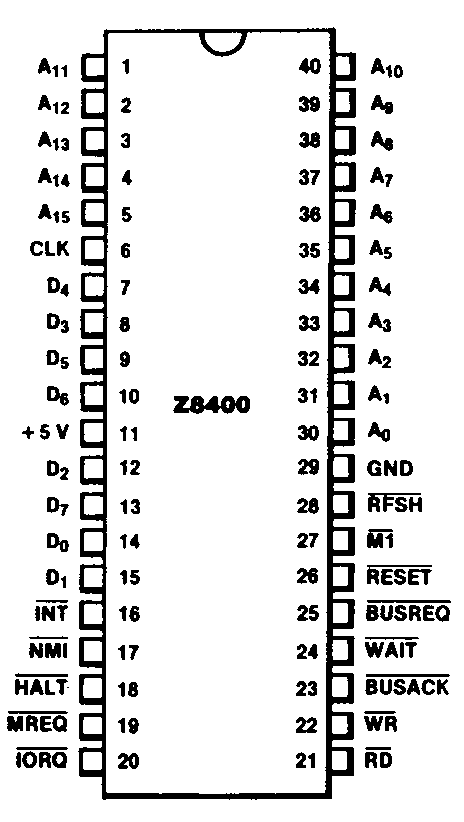
\includegraphics[width=.25\linewidth]{Reischl/img/z80-cpu-pinning-1}}\qquad
    \subfloat{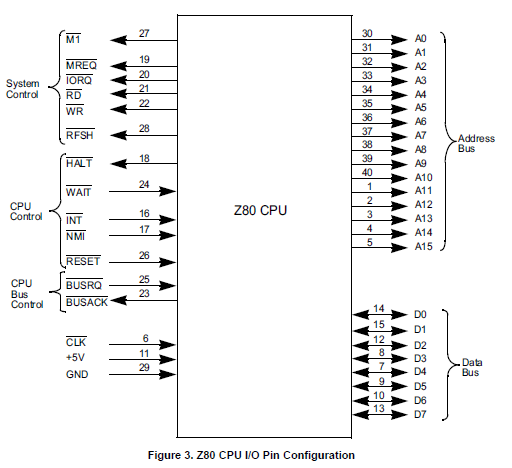
\includegraphics[width=.6\linewidth]{Reischl/img/z80-cpu-pinning-2}}\qquad
    \caption[Z80 CPU Pinning]{CPU Pinning}
    \label{fig:z80-cpu-pinning}
\end{figure}

\subsubsection{Funktionsweise und Blockschaltbild}
\fig{z80-cpu-bsb}{Z80 CPU Blockschaltbild}{CPU Blockschaltbild}{\textwidth}{Reischl/img/z80-cpu-bsb}
Bei der Z80 CPU handelt es sich um einen 8 Bit Microcontroller, der aufbauend auf dem Intel 8080 von Zilog (Frederico Faggin und Ralph Ungermann) entwickelt wurde. Der Z80 ist eine Von-Neumann Architektur, welche als CISC-Maschine (Complex Instruction Set Computer) ausgeführt ist. Die Architektur besteht aus einer Steuereinheit, welche für das Laden und Ausführen von Befehlen beziehungsweise für die Erzeugung der Steuersignale zuständig ist, einer Registerbank und einer Recheneinheit, deren zentrales Element die ALU, die Arithmetic Logic Unit, bildet. Die Kommunikation mit der Peripherie erfolgt über einen 16Bit-Adressbus, einen 8Bit breiten Datenbus und den Steuerbus. Der Speicher wird für Programmcode und Daten gleichzeitig genutzt, gleiches gilt für den Datenbus. Programmiert wird der Z80 in Assemblersprache, wobei die Befehle zwischen 1 und 4 Byte lang sein können. Die Ausführung nimmt je nach Art des Befehls zwischen einem und 5 Zyklen in Anspruch.

Das gesamte Minimalsystem arbeitet mit einer low-aktiven (erkennbar durch die invertierten Eingänge) 5V Logik, wobei NMOS (N-type Metal-Oxide Semiconductor) -, CMOS (Complementary Metal-Oxide Semiconductor)- und TTL(Transistor-Transistor Logik)-Technologie verwendet wird. Alle auf Feldeffekttransistoren basierenden Baugruppen sind TTL-kompatibel.

\subsection{PIO -- Parallel Input/Output Controller}
\subsubsection{Pinning}
\begin{figure}[htb]
    \subfloat{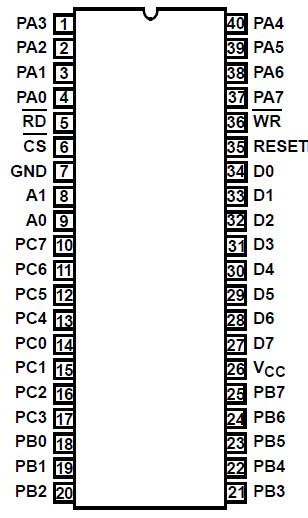
\includegraphics[width=.25\linewidth]{Reischl/img/z80-pio-pinning-1}}\qquad
    \subfloat{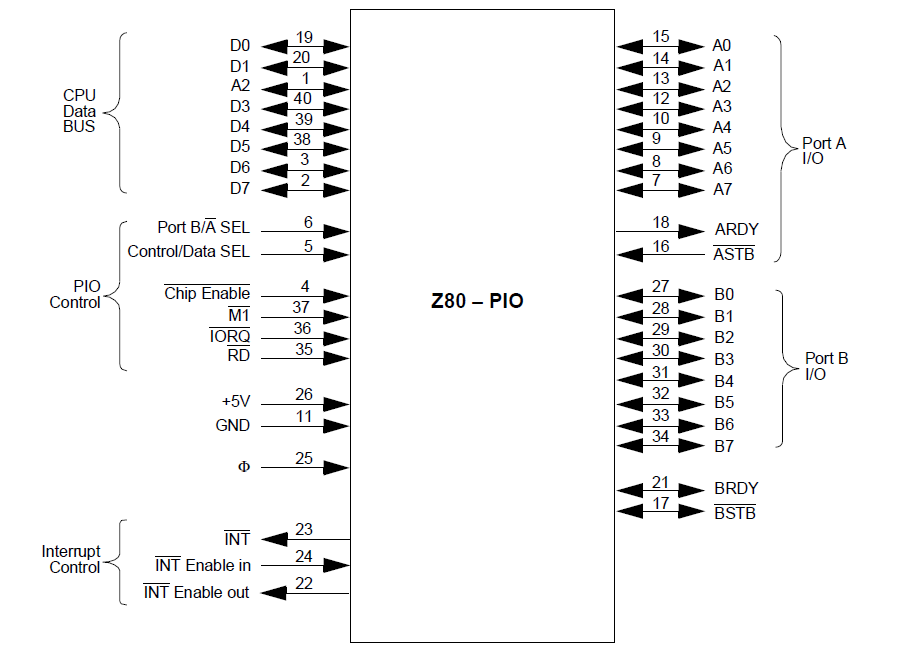
\includegraphics[width=.6\linewidth]{Reischl/img/z80-pio-pinning-2}}\qquad
    \caption[Z80 PIO Pinning]{8255 PIO Pinning \cite{z80:pio}}
    \label{fig:z80-pio-pinning}
\end{figure}

\subsubsection{Blockschaltbild und Funktionsbeschreibung}
\fig{z80-pio-bsb}{Z80 PIO Blockschaltbild}{8255 PIO Blockschaltbild \cite{z80:pio}}{\textwidth}{Reischl/img/z80-pio-bsb}
Der 82C55 ist ein von Intel entwickelter Interface-Baustein, welcher als paralleler I/O Port fungiert, deshalb die Bezeichnung PIO. Als solcher bildet er die Schnittstelle zwischen Ein- oder Ausgabeeinheit und Datenbus. Der PIO besitzt 3 Ports zu je 8 Portleitungen, somit können also insgesamt 24 Ein-/Ausgänge angesprochen werden. Mithilfe des 8255 können die an den einzelnen Ports angeschlossenen Ein- und Ausgabeeinheiten adressiert werden und ein Datenaustausch erfolgen, da jeder Port seine eigene Adresse besitzt. Um die verschiedenen Betriebsmodi der Ports anwenden zu können, muss die entsprechende Konfiguration in die Control Register des PIO geladen werden. In den Control Registern wird nicht nur die Konfiguration der einzelnen Ports gespeichert, die Control Units steuern auch die Abläufe der Zugriffe auf den jeweiligen Port und anhand von Read und Write, ob gelesen oder geschrieben wird. Details der Konfiguration können dem der Analyse des Bustimings beigefügten Erklärung, dem Datenblatt des verbauten Bausteins oder dem \textit{Z80 Family CPU Peripherals User Manual \cite{z80:periph}} entnommen werden.

\subsection{SIO -- Serial Input/Output Controller}
\subsubsection{Pinbelegung}
\begin{figure}[htb]
    \subfloat{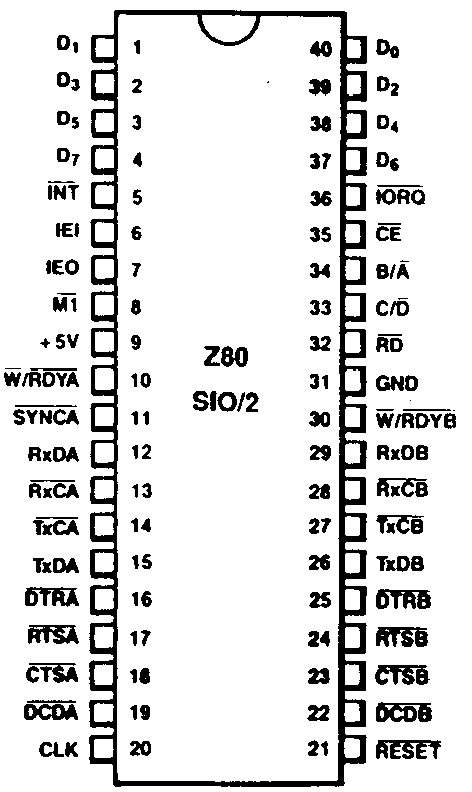
\includegraphics[width=.25\linewidth]{Reischl/img/z80-sio-pinning-1}}\qquad
    \subfloat{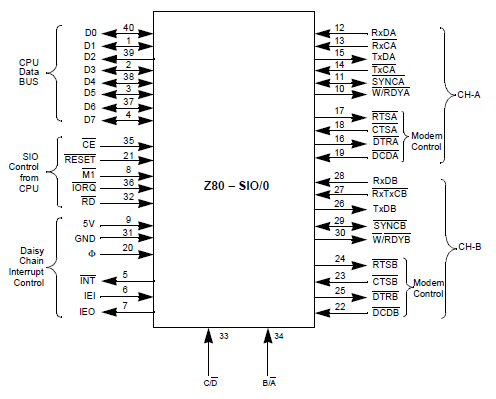
\includegraphics[width=.6\linewidth]{Reischl/img/z80-sio-pinning-2}}\qquad
    \caption[Z80 SIO Pinning]{SIO Pinning \cite{z80:sio}}
    \label{fig:z80-sio-pinning}
\end{figure}

\subsubsection{Blockschaltbild und Funktionsbeschreibung}
\fig{z80-sio-bsb}{Z80 SIO Blockschaltbild}{SIO Blockschaltbild \cite{z80:sio}}{\textwidth}{Reischl/img/z80-sio-bsb}
Der SIO dient dazu, dass die Z80 CPU über serielle Schnittstellen Daten austauschen kann. Der Baustein trägt die Bezeichnung Z84C40, das verwendete Modell Z84C4006, und wurde von Zilog entwickelt. Der Serial Input/Output Controller verfügt über 2 Kanäle, es können also bis zu 2 serielle Schnittstellen genutzt werden. Als Seriell/Parallel-Parallel/Seriell Konverter kann der SIO synchrone als auch asynchrone Protokolle verarbeiten. Um eine Kommunikation etwa über RS232 zu ermöglichen, muss die CPU während des Betriebs lediglich die Anweisung, ob geschrieben oder gelesen werden soll und etwaige zu übertragende Daten an den PIO senden, das Format der Übertragung und die Übertragungsrate wird in der voreingehenden Konfiguration festgelegt. Nähere Informationen zur Konfiguration sind dem entsprechenden Unterkapitel im Kapitel Software und Bustiming zu entnehmen beziehungsweise dem \textit{Z80 Family CPU Peripherals User Manual \cite{z80:periph}}.

\subsection{CTC -- Counter Timer Circuit}
\subsubsection{Pinning}
\begin{figure}[htb]
    \subfloat{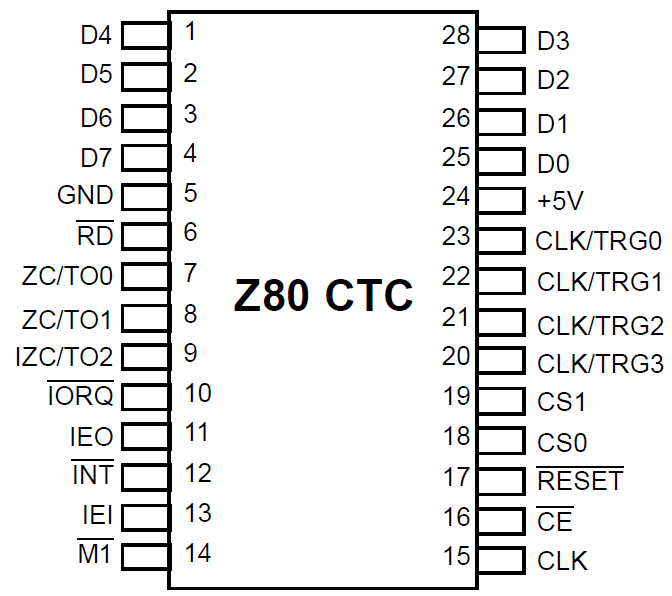
\includegraphics[width=.4\linewidth]{Reischl/img/z80-ctc-pinning-1}}\qquad
    \subfloat{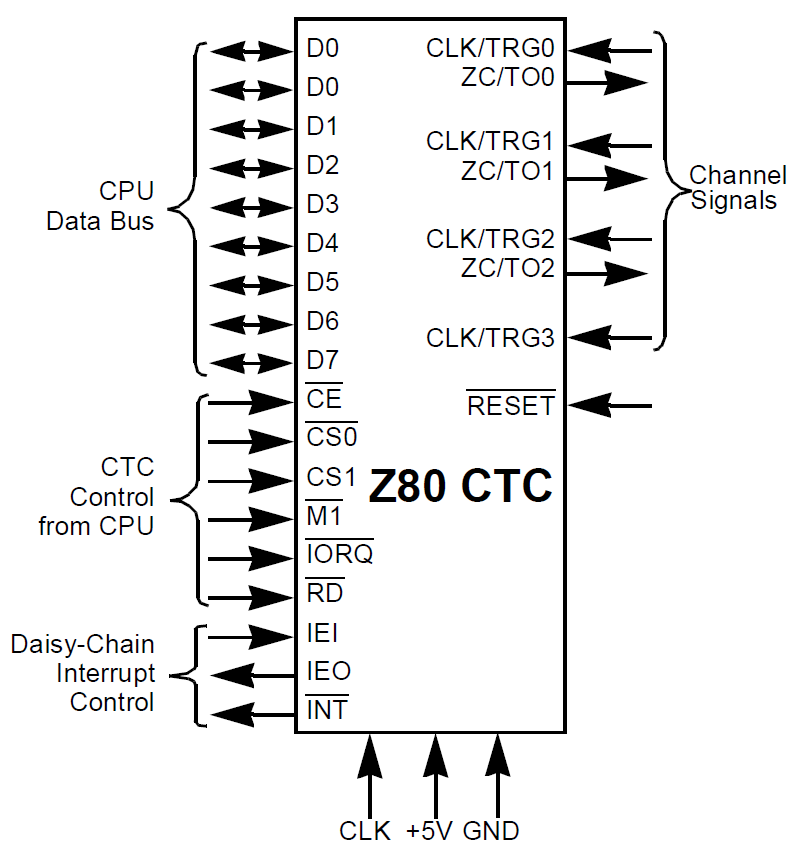
\includegraphics[width=.4\linewidth]{Reischl/img/z80-ctc-pinning-2}}\qquad
    \caption[Z80 CTC Pinning]{CTC Pinning \cite{z80:ctc}}
    \label{fig:z80-ctc-pinning}
\end{figure}

\subsubsection{Blockschaltbild und Funktionsbeschreibung}
\fig{z80-ctc-bsb}{Z80 CTC Blockschaltbild}{CTC Blockschaltbild \cite{z80:ctc}}{\textwidth}{Reischl/img/z80-ctc-bsb}
Beim Counter Timer Circuit handelt es sich um einen Baustein für die Steuerung von zeitabhängigen Vorgängen. Der Z80 CTC trägt die generelle Bezeichnung Z84C30, der verwendete Baustein 84C3006PEG. Der CTC besitzt grundsätzlich 3 verschiedene Funktionen, nämlich den Betrieb als Zähler, als Counter und die Fähigkeit, Interrupts auszulösen. Intern verfügt der Counter Timer Circuit über insgesamt 4 Kanäle, jeder dieser Kanäle besitzt einen Zähler, der in 2 verschiedenen Modi betrieben werden kann, als Zähler und als Timer. Für die Konfiguration und die Steuerung der internen Abläufe ist die Steuerlogik zuständig, das Interrupt Handling und das Erzeugen solcher wird durch die Interrupt Logik vorgenommen.

Als Zähler arbeitet das System synchron mit dem Systemtakt, also abhängig von dessen Taktflanken, wobei die höchstmögliche Zählfrequenz der Frequenz des Systemtaktes entspricht. Der Zähler ist ein Downcounter, wird 0 erreicht, wird je nach Konfiguration der Inhalt des Zeitkonstantenregisters neu geladen und ein Interrupt ausgelöst. So wie der Zähler neben dem Systemtakt auch Ereignisse am Pin TRGx (welcher beim Z80 Minimalsystem nicht beschalten, aber auf einer Stiftleiste herausgeführt wurde) des jeweiligen Kanals zählen kann, kann auch im Timerbetrieb dieser Eingang genutzt werden, um den Timer zu starten. Der Timer zählt die Impulse des Systemtakts nach dem Prescaler, der den Takt entweder um den Faktor 16 oder 256 teilt. Beim Nulldurchgang des Zählers wird der Downcounter des Timers aus dem Zeitkonstantenregister neu geladen, ein Signal am Pin ZC/TOx des jeweiligen Kanals erzeugt und bei Bedarf ein Interrupt generiert.

Die Konfiguration des CTC erfolgt mittels fix adressierter 8-Bit Datenpakete und ist vergleichbar mit der aller anderen systemspezifischen Peripherieeinheiten, genauere Informationen sind dem Kapitel Software und Analyse zu entnehmen.

\fig{z80-ctc-kan}{Z80 CTC Kanal}{Aufbau eines CTC-Kanals \cite{z80:ctc}}{0.75\textwidth}{Reischl/img/z80-ctc-kan}

\subsection{EEPROM -- Erasable Programmable ReadOnly Memory}
\subsubsection{Pinning}
\fig{z80-eprom-pinning}{Z80 EEPROM Pinning}{EEPROM Pinning \cite{z80:eprom}}{0.4\textwidth}{Reischl/img/z80-eprom-pinning}

\subsubsection{Funktionsweise}
\fig{z80-eprom-cell}{Z80 Aufbau einer Speicherzelle}{Aufbau einer Speicherzelle \cite{z80:eprom}}{0.5\textwidth}{Reischl/img/z80-eprom-cell}
Beim EPROM handelt es sich um einen 32kiB großen NMOS Flash-Speicher, welcher beim Z80 Minimalsystem als Programm- und Datenspeicher dient und von diversen Herstellern wie etwa ST Microelectronics, NEC oder Intel gefertigt wurde bzw. immer noch wird. Organisiert ist der 27256 EPROM als 32k *8, es können also 32768 Wörter zu je 8 Bit über den 15 Bit breiten Adressbus und den Steuerbus angesprochen und über den 8Bit-Datenbus abgerufen werden. Die Programmierung des EPROMS wird nicht direkt am Minimalsystem ausgeführt, sondern mit einem Programmiergerät, in welches der Speicher eingespannt wird.

\subsection{SRAM -- Static Random Access Memory}
\subsubsection{Pinning}
\fig{z80-sram-pinning}{Z80 SRAM Pinning}{62256 SRAM Pinning \cite{z80:ram}}{0.4\textwidth}{Reischl/img/z80-sram-pinning}

\subsubsection{Funktionsbeschreibung und Blockschaltbild}
\fig{z80-sram-bsb}{Z80 SRAM Blockschaltbild}{62256 SRAM Blockschaltbild \cite{z80:ram}}{0.5\textwidth}{Reischl/img/z80-sram-bsb}
Der SRAM ist ebenfalls wie der EPROM 32kiB groß und als 32k x 8 Speicher organisiert. Da der RAM im Gegensatz zum EPROM während des Betriebes des Minimalsystems auch beschrieben werden kann, wird anhand des Steuerbusses entschieden, ob Daten abgefragt oder abgespeichert werden, dabei muss der Chip immer enabled sein, es kann und darf aber immer nur entweder der Ausgang oder der Eingang aktiviert werden.

\subsection{DMA-Controller -- Direct Memory Access Controller}
\subsubsection{Pinning}
\begin{figure}[htb]
    \subfloat{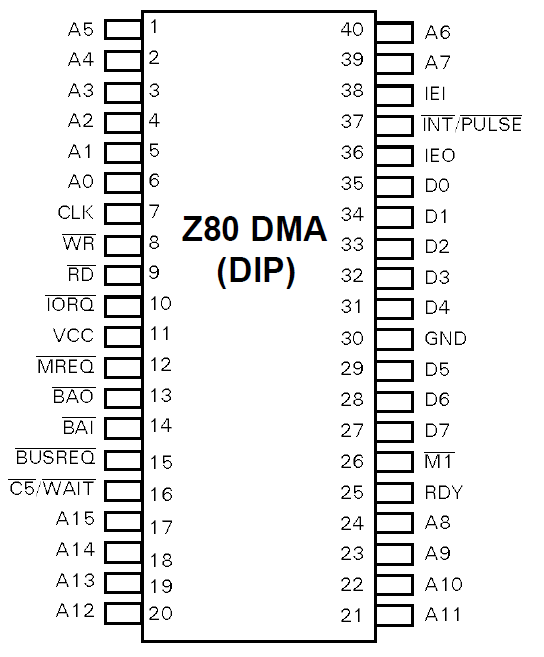
\includegraphics[width=.4\linewidth]{Reischl/img/z80-dma-pinning-1}}\qquad
    \subfloat{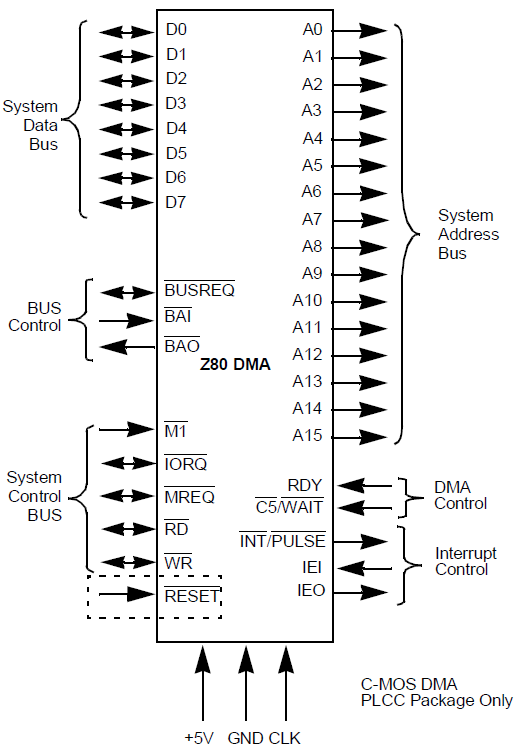
\includegraphics[width=.4\linewidth]{Reischl/img/z80-dma-pinning-2}}\qquad
    \caption[Z80 DMA Pinning]{DMA Pinning \cite{z80:dma}}
    \label{fig:z80-dma-pinning}
\end{figure}

\subsubsection{Funktionsbeschreibung und Blockschaltbild}
\fig{z80-dma-bsb}{Z80 DMA Blockschaltbild}{DMA Blockschaltbild \cite{z80:dma}}{\textwidth}{Reischl/img/z80-dma-bsb}
Der DMA Controller ist ein für den Z80 und den Z8000 entwickelter IC mit der Bezeichnung Z8410 oder Z84C10 bei der Verwendung von MOSFET-Halbleitern und ermöglicht einen Speicherdirektzugriff, es werden die Daten also nicht mithilfe der CPU aus dem Speicher geholt und dann von der CPU an die entsprechende Peripherieeinheit übermittelt, sondern direkt zwischen dem Speicher und der jeweiligen Peripherieeinheit ausgetauscht. Diese direkte Kommunikation der Peripheriegeräte mit dem Speicher ist performanter als der Datentransfer via CPU, da ein Zwischenspeichern in den Registern der CPU und ein Instruction Fetch bei jedem Transfer wegfällt. Neben dem Datentransfer zwischen den 2 Ports des DMACs besteht auch die Möglichkeit, nach einem bestimmten Bitwort zu suchen. Die Datenübertragung wird von der CPU durch das Übertragen der ersten Adresse und über den Steuerbus (Memory Request, I/O Request, Bus Request, Acknowledge, Read, Write) gesteuert, gestartet wird der Übertragungsvorgang ebenfalls von der CPU. Der DMAC kann in 3 verschiedenen Modi betrieben werden: Im Byte- oder Single Mode steht nach jedem übertragenen Byte kann die CPU den Datenbus nutzen, im Burst Mode werden solange Daten übertragen wie der jeweilige Port des DMA aktiv ist und im Continuous Mode wird die Übertragung der Daten entweder durch das Erfüllen der Stopp-Bedingung oder durch das Erreichen des Endes des zu übertragenden Datensatzes beendet.

\subsection{NMI -- Non Maskable Interrupt}
\fig{z80-nmi-bsb}{Z80 NMI Blockschaltbild}{NMI Blockschaltbild}{0.5\textwidth}{Reischl/img/z80-nmi-bsb}
Soll ein NMI, ein nicht maskierbarer Interrupt durch den Anwender ausgelöst werden, so muss dieser den Taster S1 betätigen. Die Leitung NMI, welche mit einem Pull-Up Widerstand versehen ist, ist mit der CPU verbunden und diese löst dann einen Interrupt aus.

\subsection{CE-Logik}
\fig{z80-ce-bsb}{Z80 CE-Logik Blockschaltbild}{CE-Logik - 74LS244 Decoder Blockschaltbild}{0.5\textwidth}{Reischl/img/z80-ce-bsb}
Die CE-Logik besteht aus 2 Demultiplexern mit jeweils 4 Ausgängen, welche für das Enablen der einzelnen Bausteine, also das Aktivieren des jeweiligen CS- bzw. CE-Eingangs, zuständig ist. Die beiden Decoder bilden einen gemeinsamen Baustein, bei welchem es sich um einen Standard-IC vom Typ 74LS139 handelt. Der erste Decoder ist für die Speicher zuständig, wo er anhand von Memory Request und des 16. Bits des Adressbus SRAM oder EPROM enabled. Liegt am 16. Bit des Adressbusses 1 an, so wird der SRAM enabled, bei 0 wird auf den EPROM zugegriffen. Mit dem anderen Decoder werden die Peripherieeinheiten CTC, PIO, SIO und DMA aktiviert. Anhand des 7. Und 8. Bits des Adressbusses wird bei 00 der CTC, bei 01 der SIO, bei 10 der PIO und bei 11 der DMA Controller enabled, wobei gleichzeitig auch der I/O Request aktiviert sein muss.

\subsection{I/O Einheiten}
\subsubsection{Ausgabeeinheit}
\fig{z80-ioo-bsb}{Z80 Ausgabe LEDs}{Ausgabe LEDs}{\textwidth}{Reischl/img/z80-ioo-bsb}
Der Port A des PIO ist mit einem 8-fach LED-Array als parallele Ausgabeeinheit ausgestattet. Um den Ausgang des PIO nicht zu belasten, wird ein 8-fach Bustreiber verwendet, um die LEDs zu betreiben. Dieser Treiber wirkt invertierend und seine Ausgänge sind mit den Eingängen OE1 und OE2 mittels Jumper J3 deaktivierbar. Ist der Jumper so gesetzt, dass die LEDs versorgt werden können, leuchtet auch eine zusätzliche LED V9. Wird an den OE Eingang GND angelegt werden, würde die Arbeitsrichtung des Treiberbausteins umgekehrt werden, was aber bei dieser Anwendung keine Verwendung findet. Um die Helligkeit der LEDs von der Anzahl der aktivierten LEDs unabhängig zu machen, sind 2 Dioden in Serie zu den 8 LEDs geschaltet. Die 2 Dioden ersetzen den sonst üblichen Serienwiderstand bei jeder einzelnen LED, der Grund für 2 Dioden liegt darin, dass bei der Anwendung von einer einzelnen Diode die Spannung an den LEDs zu hoch ist und damit die Helligkeit.

\subsubsection{Eingabeeinheit}
\fig{z80-ioi-bsb}{Z80 Eingabe-Schalter}{Eingabe-Schalter}{0.75\textwidth}{Reischl/img/z80-ioi-bsb}
Die Eingabeeinheit besteht aus einem 8-fach DIP-Schalter, dessen Ausgang als Pull-Up betrieben wird. Ist ein Schalter also offen, liegen am Eingang des Port B des PIO 5V an, wird der Schalter geschlossen so liegen am entsprechenden PIN des PIO 0V an. Da es sich beim Z80 um eine Low-aktive Logik handelt, interpretiert die CPU einen offenen Schalter als logisch 0 und einen geschlossenen Schalter als 1.

\subsection{RS232 Schnittstelle}
\fig{z80-rs232-bsb}{Z80 UART-RS232}{UART-R232}{0.75\textwidth}{Reischl/img/z80-rs232-bsb}
Die RS 232 Schnittstelle wird durch den SIO gesteuert, dieser fungiert also als UART, was auch bedeutet, dass die Anzahl von Daten-, Start- und Stoppbits, die Verwendung eines Sign Bits und die Baudrate mit der Konfiguration des Ports A des Z80 SIO festgelegt werden. Der Z80 wird als Modem (DÜE – Datenübertragungseinrichtung) betreiben, das bedeutet, dass die Bezeichnung der Datenleitungen Rx (Receive Data) und Tx (Transmit Data) sind und die Steuerleitungen RTS (Request to Send) und CTS (Clear to Send) nur aus Sicht des Terminals, der DEE (Datenempfangseinrichtung) gültig. Da zwar der UART, nicht aber RS232 mit Logikpegeln arbeitet, müssen 0V und 5V auf +/-15V mittels Pegelwandler umgesetzt werden. Diese Aufgabe übernimmt der MAX232.

\subsection{Pull-Ups}
\fig{z80-pu-bsb}{Z80 Pull-Ups}{Pull-Ups}{\textwidth}{Reischl/img/z80-pu-bsb}
Da alle Eingänge der Busse als Pull-Up Eingänge ausgeführt sind, ist es notwendig, alle Leitungen der Busse, deren Zustand bei Nichtbenutzung nie ungleich Null sein darf, mit einem Widerstand von in diesem Fall 10k$\Omega$ gegen Betriebsspannung = 5V zu versehen. Dies geschieht am Einfachsten mit Widerstands-Arrays, wo intern 8 Widerstände parallel gegen einen einzelnen Pin geschalten werden, welcher dann mit der Betriebsspannung verbunden wird. Das Z80 Minimalsystem besitzt solche Widerstandsarrays für den Daten- und für Teile des Steuerbusses.

\section{Troubleshooting}
\label{sec:z80-troubleshooting}
\subsection{Spannungsversorgung}
Im Vergleich zu den Vorgängerversionen wurde die Spannungsversorgung stark modifiziert. Beim Z80 Minimalsystem V4.5 wurde eine Leiterbahnbreite von unter 25 Mil = 0,64mm für die Versorgungsleitungen vorgesehen, welche bei der Verwendung von alter TTL-Komponenten, wo der Stromverbrauch abhängig vom angewendeten Programm 400 bis zu 440 mA beträgt, zu einem Spannungsabfall von 0,6V zwischen Linearregler und 5V Pin der CPU führen. Es kann das in den Datenblättern vorgegebenen Minimum von 4,75V nicht erreicht werden, der gemessene Spannungswert an den herausgeführten Pins der CPU ergibt eine Spannungsdifferenz von minimal 4,35V. Bei der aktuellen Version 4.9 werden die Leiterbahnen für 5V und Ground mit mindestens 50 mil Breite ausgeführt, ebenso wird die Schottky-Diode, welche als zusätzlicher Verpolungsschutz dient, durch eine Parallelschaltung zweier Schottky-Dioden zur Minimierung der Spannung an der Diode ersetzt. Als Ergebnis dieser Überdimensionierung erhält man eine Spannung von mindestens 4,75V an der Versorgung der CPU, auch dann, wenn TTL- anstatt CMOS- oder NMOS-Technologie eingesetzt wird.

Neben vielen kleineren Änderungen sollte der Wechsel von Micro USB auf USB Typ B erwähnt werden. Durch diese Änderung wird die mechanische Stabilität des Steckers wesentliche verbessert und dadurch Störfälle minimiert.

\subsection{Reset}
Der Reset wurde ursprünglich ohne die Verwendung von Schmitt-Triggern zur Stabilisierung des Signals beschaltet, was sehr viele kurze Störimpulse durch das Prellen des Schalters zur Folge hatte. Durch die nunmehrige Anwendung eines Kondensators zum Vermeiden von Spannungssprüngen in Kombination mit 2 Schmitt-Trigger-Invertern und einem D-Flip-Flop ergibt sich eine Ladekurve mit einer Zeitkonstante von rund 60ms und daraus ein sauberer Reset-Impuls.
\fig{z80-reset-oszi}{Z80 Resetimpuls}{Resetimpuls}{0.75\textwidth}{Reischl/img/z80-reset-oszi}

\subsection{Taktsignal}
Das Taktsignal wirkt sich nicht negativ auf die Funktion des Minimalsystems aus, doch weist es noch immer unerwünschte Impulse und die Pegel des Systemtaktes weichen von den Vorgaben des Datenblattes der CPU ab. Abhilfe würde durch die Verwendung von SMD-Widerständen aufgrund geringerer parasitärer Größen und den Wechsel auf schnellere CMOS-Gatter für die Takterzeugung schaffen. Die Gatter vom Typ HTC bzw. AHCT weisen kürzere Schaltzeiten auf, besitzen jedoch die gleichen Schwellen wie die TTL-Gatter vom Typ LS.
\fig{z80-takt-oszi}{Z80 Taktsignal}{Taktsignal}{0.75\textwidth}{Reischl/img/z80-takt-oszi}

\section{Programmierung}
\label{sec:z80-programmierung}
\subsection{Programmierung des EPROMs}
Die Programmierung des EPROMS wird mit einem Programmiergerät vorgenommen. Dieses Programmiergerät wird mittels USB mit einem Computer verbunden. Um die Software MiniPro Programmer für das Programmiergerät zu installieren, muss die beigefügte CD ausgeführt werden. Bei der Installation können die Standardeinstellungen übernommen werden. Ist die Installation ausgeführt worden, müssen nur noch die Speicherzellen entsprechend der vorgesehenen Adressierung mit Intel HEX Code befüllt werden.
\fig{z80-programmierung-eprom}{Z80 EPROM Programmierung - Mini Pro V6.10}{EPROM Programmierung - Mini Pro V6.10}{\textwidth}{Reischl/img/z80-programmierung-eprom}

\subsection{Z80 Assembler}
Grundsätzlich kann die Übersetzung des Assemblercodes in Intel HEX-Code von Hand erfolgen. Bei größeren Programmen empfiehlt es sich, einen Assembler zu verwenden, wie etwa das Crossware Embedded Development Studio, welcher sowohl als Assembler als auch als Simulator verwendet werden kann. Da dieser Assembler auf die Anwendung mit dem MPF 1B ausgelegt wurde, muss die Startadresse auf 0000 statt 1800 geändert werden ebenso wie die Größe des Speichers und die Auswahl des EPROMS als Programmspeichermedium. Genaue Informationen zu Installation und Anwendung liegen der Software in englischer Sprache bei.

\section{Kostenrechnung}
\label{sec:z80-kostenrechnung}
Kosten für die Fertigung von 5 PCBs bei PCBWay inklusive Frachtkosten:
60 \$ = 48,60 €

Fertigungskosten für ein Minimalsystem (alle Preise Stand März 2018):
\begin{itemize}
    \item PCB: 9,72 €
    \item Bauteile: 75,50 €
    \item Summe: 85,22 €
\end{itemize}

\section{Software und Analyse}
\label{sec:z80-software}
\subsection{Beschreibung der Hardware}
Eine genaue Beschreibung der Hardware ist dem Kapitel Aufbau des Z80 Minimalsystems und Beschreibung der Baugruppen zu entnehmen.

\subsection{Der Von-Neumann Zyklus}
Der von-Neumann-Zyklus, benannt nach dem österreich-ungarischen, später US-amerikanischen Mathematiker János/Johann/John von Neumann, beschreibt den Ablauf der Befehlsverarbeitung in einer entsprechend den Vorschlägen von Neumanns entworfenen Architektur. Diese besteht wie bereits im vorherigen Punkt beschrieben aus einer ALU (Arithmethic Logic Unit), dem Rechenwerk, einer Control Unit, dem Steuerwerk, einem Bussystem, einem Speicherwerk, welches sowohl Daten als auch Instruktionen gleichwertig speichert und den Ein- und Ausgabeeinheiten. Die Befehlsausführung wird in 5 Schritten vorgenommen:

\begin{enumerate}
    \item \textbf{Instruction Fetch}: Instruktion aus den EPROM in das Befehlsregister laden.
    \item \textbf{Instruction Decode}: Der Befehlsdecoder decodiert den HEX-Code aus dem Befehlsregister, sodass der Controller Sequenzer die nötigen Steuersignale erzeugen kann.
    \item \textbf{Operanden Fetch}: Entsprechend dem decodierten Befehl werden die geforderten Operanden aus dem Speicher geladen.
    \item \textbf{Execute}: Ausführung des Befehls.
    \item \textbf{Write Back}: Die erhaltenen Ergebnisse werden, wenn notwendig in die Register oder in den Arbeitsspeicher zurückgeschrieben.
\end{enumerate}
Im Fall des Z80 ist jeder Zyklus 10 Takte lang, das ergibt bei einer Taktrate von 1,864MHz eine Dauer von 5,36$\mu$s.

\subsection{Vorbereitung zur Analyse der Z80-Befehlsabarbeitung}
\subsubsection{Installation der DigiView-Software}
Um die mittels Logikanalysator aufgenommenen Signalverläufe auf einem PC anzeigen zu können bzw. die Analyse durchzuführen, muss das Programm DigiView installiert werden, welche auf der dem Logikanalysator beigelegten Installations-CD enthalten ist. Bei der Installation der Software muss nach der vorgenommenen Installation noch der Treiber für den Logikanalysator nachinstalliert werden. Dies geschieht üblicherweise über die Systemsteuerung, wo als Quelle für den Treiber die CD zu wählen ist.

\subsubsection{Kanalkonfiguration in DigiView}
\label{sec:z80-digiview-kanal}
Um die Signale erfassen und analysieren zu können, muss für jeden einzelnen Kanal, also für jeden Eingang des Logikanalysators, eine Bezeichnung vergeben werden. Für die anschließende Analyse muss festgelegt werden, um welche Art von Signal es sich handelt. Grundsätzlich wird zwischen einzelnen Leitungen (Boolean) und zwischen einem Bündel von Leitungen (Bus) unterschieden.

Konfiguration für das Programm PIO Test \#2:
\fig{z80-digiview-kanal}{Z80 DigiView Kanalkonfiguration PIO Test 2}{DigiView Kanalkonfiguration PIO Test 2}{\textwidth}{Reischl/img/z80-digiview-kanal}
Anmerkung: Diese Belegung ist beispielhaft und entspricht nur der Belegung der Kanäle zur Erfassung des Bustimings des Programms PIO\_TEST\#2. Die erfassten Signale bzw. die Auswahl und Belegung der Kanäle unterscheidet sich bei den jeweiligen Programmen, weshalb sie bei jedem Einzelnen separat angeführt ist.

\subsubsection{Festlegung der Triggerbedingung in DigiView}
Für das Auslösen des Aufzeichnungsvorgangs muss wie bei einem Oszilloskop ein Trigger gesetzt werden. Dieser Trigger wird als Hardware Trigger ausgeführt, die Triggerung wird mittels logischer Verknüpfung eines oder mehrerer Kanäle unter dem Menüpunkt Config $\rightarrow$ Trigger erstellt.
\fig{z80-digiview-trigger}{Z80 DigiView Trigger}{DigiView Trigger}{\textwidth}{Reischl/img/z80-digiview-trigger}
Die in der obigen Abbildung dargestellte Trigger-Bedingung besteht aus 3 Elementen: Der erste Teil der Bedingung wird erfüllt, sobald der Kanal Reset, welcher dem Ausgang der Reset-Schaltung des Minimalsystems entspricht, für eine Zeit von mindestens 10us (Minimum: 3 Taktzyklen entspricht 1,61us) LOW ist. Folgt darauf eine positive Flanke und ein HIGH von 10us, so sind auch der 2. und 3. Teil der Bedingung erfüllt, der Trigger wird ausgelöst und die Aufzeichnung startet. Der erste und zweite Teil der Bedingung vermeiden, dass der Logikanalysator auf ein Störsignal triggert, der dritte Teil prüft auf unerwünschte, störungsbedingte Reset-Impulse und ist nicht zwingend erforderlich.

\subsection{Verbindung des Logikanalysators mit dem Z80 Minimalsystem}
Der Logikanalysator, welcher in der Laborübung verwendet wird, besitzt 36 Kanäle, die über 2 Stecker mit jeweils 18 Kanälen und 2 Masseverbindungen nach außen geführt werden. Die einzelnen Leitungen besitzen eine festgelegte farbige Markierung, um die Zuordnung zu erleichtern.

Messleitungen/Kanäle des Logikanalysators:
\fig{z80-digiview-logik}{Z80 DigiView Kanäle des Logikanalysators}{DigiView Kanäle des Logikanalysators}{\textwidth}{Reischl/img/z80-digiview-logik}
Entsprechend dieser Zuordnung und der zuvor festgelegten Kanäle müssen die herausgeführten Pins von Adressbus, Datenbus, CE-Logik und der Steuerleitungen des Z80 Minimalsystems mit den Leitungen der einzelnen Kanäle verbunden werden.
Die Zuordnung der auf die Stiftleisten herausgeführten Leitungen kann entsprechend dem Aufdruck auf der Platine und den Schaltplänen vorgenommen werden, es sollte aber dringend darauf geachtet werden, dass auch GND (fixe Belegung am Logikanalysator, bezeichnet mit G) verbunden wird.

\subsubsection{Belegung der herausgeführten Leitungen auf dem Minimalsystem}
\begin{warning}
Anmerkung: Um etwaige Fehler bei der späteren Interpretation der Timing Diagramme zu vermeiden, sollte angemerkt werden, dass es sich bei dem Z80 Minimalsystem um eine low-aktive Logik handelt.
\end{warning}
\begin{figure}[htb]
    \centering
    \subfloat{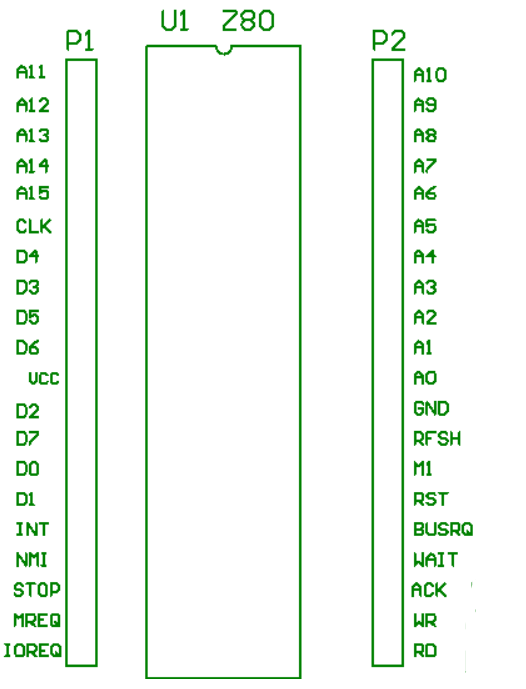
\includegraphics[width=.28\linewidth]{Reischl/img/z80-stiftleiste-1}}\qquad
    \subfloat{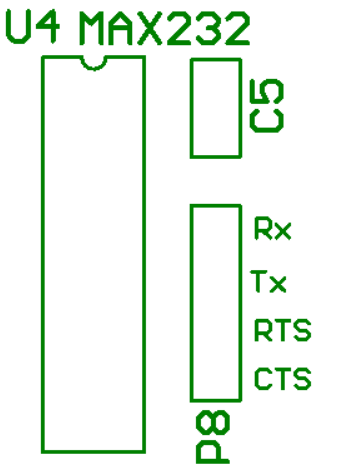
\includegraphics[width=.28\linewidth]{Reischl/img/z80-stiftleiste-2}}\qquad
    \subfloat{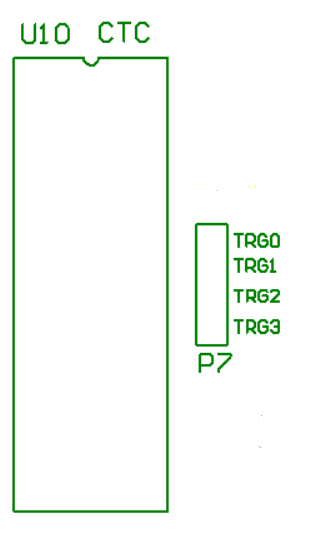
\includegraphics[width=.28\linewidth]{Reischl/img/z80-stiftleiste-3}}\qquad
    \caption[Z80 Belegung der Stiftleisten an CPU, CTC und UART]{Belegung der Stiftleisten an CPU, CTC und UART}
    \label{fig:z80-stiftleiste}
\end{figure}

\subsection{PIO Testprogramm}
\subsubsection{Aufgabenstellung}
Es ist mithilfe eines Logikanalysators der Befehlsablauf einer Von-Neumann-Architektur anhand des Z80 Minimalsystems zu analysieren. Das zu verwendende Programm für den Zilog Z80 lautet auf dem Namen PIO\_TEST\#2, es liest mithilfe des PIO (8255) die Schalterstellung aus und zeigt diese über die LEDs an. Es soll eine Erfassung des Befehlsablaufes ab dem Reset vorgenommen werden, anschließend zu analysieren sind vor allem die Instruktionen, die in das Control-Register des PIO geschrieben werden. Weiters soll eine Messung der Zugriffszeiten auf die einzelnen Komponenten des Systems, in diesem Fall auf EPROM und PIO, erfolgen und die Gatterlaufzeit der CE-Logik ermittelt werden.

\subsubsection{Source Code}
Das Programm für den Z80 wird in Assemblersprache verfasst. Um das Programm ausführen zu können, muss die Assemblersprache in Hex-Code übersetzt werden und dieser mit einem Programmiergerät in ein EPROM geschrieben werden.

\subsubsubsection{Assemblerbefehle}
\lstinputlisting[language={[Z80]Assembler}, caption=Z80 PIO Test, label=lst:z80-pio]{Reischl/lst/pio.s}

\subsubsubsection{Funktionsbeschreibung}
Um den Zugriff der CPU auf die Ein- und Ausgabeeinheiten und die dort angeschlossenen Sensoren und Aktoren zu ermöglichen, wird der PIO benötigt, welcher die Daten einliest und über den Datenbus verschickt bzw. die Daten, die er über den Datenbus erhält, an den entsprechenden Port und die dort angeschlossene Peripherieeinheit anlegt. Die Adressen für die einzelnen Ports des PIO werden diesem Programm als Konstanten vordefiniert. Das Programm selbst lädt zuerst die Konfiguration des PIO Controllers, dann liest er die Schalterstellung des DIL-Schalters in einer Endlosschleife ein und gibt die Schalterstellung über die LEDs aus.

\subsubsection{Konfiguration des PIO}
Der Port B des Parallel Input/Output Controllers soll als Output für die Ausgabe über LED konfiguriert werden, Port A als Input für das Einlesen der Schalterstellungen des DIL-Schalters. Die Konfiguration erfolgt durch Senden der Konfiguration an die Adresse des Steuerregisters.
\fig{z80-pio-konf}{Z80 Konfiguration PIO}{Konfiguration PIO 8255 \cite{z80:pio}}{0.5\textwidth}{Reischl/img/z80-pio-konf}
Konfiguration:
\begin{enumerate}
    \item D0: 1: Port C (C0 bis C3) als Output (nicht in Verwendung)
    \item D1: 0: Port B als Output 
    \item D2: 0: Mode 0 
    \item D3: 1: Port C (C4 bis C7) als Output (nicht in Verwendung)
    \item D4: 1: Port A als Input
    \item D5 \& D6: Mode 0
    \item D7: 1: Modus wird als aktiv gesetzt
\end{enumerate}

\subsubsection{Konfiguration des Logikanalysators}
Die Kanalbelegung des Logikanalysators ist der Erläuterung der Bedienung des Logikanalysators in \fref{sec:z80-digiview-kanal} zu entnehmen.

\subsubsection{Analyse}
Die Beschreibung der einzelnen Zyklen erfolgt entsprechend der Bezeichnung der einzelnen Marker T, A-D, X und Y.
\fig{z80-digiview-pio}{Z80 DigiView PIO Test 2 Teil 1}{DigiView PIO Test 2 Teil 1}{\textwidth}{Reischl/img/z80-digiview-pio}
Marker T: Mit dem Reset wurde der Programm Counter auf die Adresse 0000 zurückgesetzt. Die Adresse 0000 ist als die erste Adresse des auszuführenden Programms festgelegt, weshalb die CPU einen Opcode Fetch durchführt. Dass ein Befehl zur Ausführung aus dem Speicher geholt wird, wird durch die Leitung M1 (Machine Cycle One) angezeigt. Die richtige Adresse für den ersten Befehl liegt bereits auf dem Datenbus an, also muss nur noch die Datenabfrage aus dem ROM ermöglicht werden. Dafür wird von der CPU ein Memory Request und ein Read ausgelöst und die CE-Logik enabled den EPROM. Dieser legt nun die Daten der Speicherzelle 0000 an den Datenbus. Von dort liest die CPU den Befehl ein und lädt ihn in den Befehlsdecoder, welcher den Hex-Code decodiert. Der erhaltene Befehl lädt eine Konstante in den Akkumulator.

Marker A: Nach einem Refresh, welcher für das Halten der Daten im RAM verantwortlich ist, wird an den Adressbus die Adresse 0001 angelegt. Die CPU sendet wiederum einen Memory Request und ein Read, bereitet also einen Lesevorgang vor. Die CE-Logik ermittelt den EPROM als Quelle der angefragten Daten und enabled diesen. Der ROM legt den Inhalt der Speicherzelle 0001 an den Datenbus an, die CPU kann die Konstante 99 in den Akku laden und damit ist die Ausführung des ersten Befehls abgeschlossen. Die in den Akku geladene Konstante ist für die Konfiguration des PIOs (8255) bestimmt, die Details der Konfiguration sind dem entsprechenden Kapitel zu entnehmen. Der Port B des Parallel Input/Output Controllers soll als Output für die Ausgabe über LED konfiguriert werden, Port A als Input für das Einlesen der Schalterstellungen des DIL-Schalters, als Modus wir der Mode 0 gewählt.

B: Der zweite auszuführende Befehl liegt auf der Adresse 0002, für das Einlesen der Instruktion wird wiederum von der CPU ein Machine Cycle One (M1), ein Memory Request und ein Read erzeugt und von der CE-Logik der EPROM ausgewählt. Der Assemblerbefehl ist für die Ausgabe des Inhalts des A-Registers, des Akkus, an eine fix vorzugebende Adresse zuständig, der dazugehörige Hex-Code, der auf dem Datenbus anliegt, lautet D3.

C: Auf der Adresse 0003 liegt die Zieladresse des Ausgabebefehls, für die Ausgabe der Adresse 83 liefert die CPU ein Memory Request und ein Read, die Chip-Select-Logik wählt den EPROM aus.

D: Das Control Register des PIO wird mit 9983 adressiert, wobei mit den ersten beiden Bits (A0 und A1) im PIO ermöglicht wird, dass das Datenwort in das Control-Register geschrieben wird. Für das Laden der Konfiguration sendet die CPU ein Write und einen I/O-Request, die CE-Logik wählt den PIO als Ziel der Information aus.

X: Der Programm Counter legt die Adresse 0004 an den Adressbus an. Sa es sich um den nächsten Befehl handelt, wird dies durch den aktiven Port M1 angezeigt, ebenso erzeugt die CPU einen Memory Request und ein Read und die CE-Logik, ein doppelter Vierfach-Demultiplexer, selektiert den EPROM. Am Datenbus liegt der Hex-Code DB an, der für einen Einlesevorgang des Inhalts einer fix festzulegenden Speicherzelle in den Akkumulator steht.

Y: Von der EPROM-Speicherzelle mit der Adresse 0005 wird die Adresse für den Einlesevorgang geladen. Dafür erzeugt die CPU einen Machine Cycle One, ein Memory Request und ein Read, die CE-Logik wählt anhand der ersten 4 Bits der Adresse (A0 bis A3) den EPROM als Quelle der Daten. Nach einer Laufzeit legt der EPROM den Inhalt der Speicherzelle, 83, an den Datenbus an.

Z: Von der an den Datenbus angelegten Adresse 9983 soll die Konfiguration des PIO gelesen werden. Dafür erzeugt die CPU ein I/O-Request und ein Read, die CE-Logik selektiert den PIO. Das erhaltene Ergebnis auf dem Datenbus lautet 99.

\fig{z80-digiview-pio-2}{Z80 DigiView PIO Test 2 Teil 2}{DigiView PIO Test 2 Teil 2}{\textwidth}{Reischl/img/z80-digiview-pio-2}
A: Am Adressbus legt der Programm Counter die Adresse 0006 an. Von dieser soll ein neuer Befehl geladen werden, was anhand des von der CPU erzeugten Machine Cycle One, des Memory Requests und des Reads beziehungsweise am von der CE-Logik gewählten EPROM ersichtlich ist. Der am Datenbus anliegende Befehl mit dem Hex-Code DB ist, wie bereits beschrieben, für das Auslesen von Peripherieeinheiten und das anschließende Speichern der ausgelesenen Information im Akku zuständig.

B: Auf der Adresse 0007 liegt im EPROM die Adresse des Ports B des PIO. Damit die CPU diese Adresse erhält, muss sie 0007 an den Adressbus legen und einen Memory Request und ein Read erzeugen. Anhand der Adresse kann die Chip-Select-Logik den EPROM als Quelle der Information auswählen und dieser gibt den Inhalt der entsprechenden Speicherzelle, die Adresse 80, über den Datenbus aus.

C: Am Adressbus liegt die Adresse 9980 an, mit welcher der Port A des PIO angesprochen wird. Um die Schalterstellungen der DIL-Schalter ermitteln zu können, generiert die CPU einen I/O-Request und ein Read, die CE-Logik enabled den PIO. Nach einer Laufzeit liefert der PIO die Schalterstellung 0A (S7 – S0: 00001010) über den Datenbus an die CPU.

D: Nachdem der vorherige Befehl ausgeführt wurde, legt der Programm Counter die Adresse 0008 an den Adressbus an, um den in der Speicherzelle mit der entsprechenden Adresse vorhandenen Befehl einzulesen, zu decodieren und ausführen zu können. Dafür erzeugt die CPU einen Machine Cycle One, einen Memory Request und ein Read, die Chip-Select-Logik wählt anhand der Adresse den EPROM. Der Befehl mit dem Hex-Code D3, der nun am Datenbus anliegt, sendet den Inhalt des Akkus, in diesem Fall 0A, an eine durch den Programmierer festzulegende Adresse.

X: Nachdem der Programm Counter inkrementiert wurde, liegt am Adressbus 0009 an. Mittels eines Speicher-Lesezugriffs (M1, MREQ, READ, CS EPROM) wird 81 als Inhalt der entsprechenden Speicherzelle und Zustelladresse der zu übertragenden Daten über den Datenbus in das Befehlsregister der CPU geladen.

Y: Für die Ausführung des Befehls wird die Adresse des PIO, A81, an den Adressbus angelegt, die CPU erzeugt einen I/O-Request und ein Write, die CE-Logik enabled den PIO. Am Datenbus liegt die aktuelle Schalterstellung, diese gibt der PIO nach einer Laufzeit über den Port B aus beziehungsweise die LEDs, deren zugehörige Bits ‚1‘ sind, leuchten auf.

\fig{z80-digiview-pio-3}{Z80 DigiView PIO Test 2 Teil 3}{DigiView PIO Test 2 Teil 3}{\textwidth}{Reischl/img/z80-digiview-pio-3}
A: Der Programm Counter wird inkrementiert, am Adressbus liegt 000A an. Da auf dem EPROM unter dieser Adresse ein neuer Befehl liegt, liefert die CPU einen Machine Cycle One, einen Memory Request und ein Read. Nachdem die CE-Logik den RAM enabled hat, legt dieser C3 als Inhalt der Speicherzelle an den Adressbus. Bei dem ins Befehlsregister der CPU geladenen Befehl handelt es sich um einen absoluten Sprungbefehl.

B: Die nächste Speicherzelle mit der Adresse 000B beinhaltet die Sprungadresse 06, welche nach mittels Speicher-Lesezugriffs an den Datenbus gelegt wird.

C: Da es sich bei dem Sprungbefehl um einen 16 Bit-Befehl handelt, wird ein weiterer Speicher-Lesezugriff durchgeführt, um auch die restlichen 8 Bit zu erhalten.

D: Nach dem Sprung liegt auf dem Adressbus wieder die Adresse 0006 an. Die CPU erzeugt einen Machine Cycle One, weiters erzeugt sie einen Speicher-Lesezugriff für das Lesen des nächsten auszuführenden Befehls. Der Befehl ist, wie bereits beschrieben wurde, für das Auslesen von Daten von einer bestimmten Adresse und das anschließende Schreiben des Ergebnisses in den Akkumulator zuständig.

X: Mittels Speicher-Lesezugriff (Memory Request, Read, Chip Enable des EPROMs) wird die festgelegte Adresse für die Datenabfrage geladen.

Y: Um die Daten vom Port A des PIO abzufragen, wird dieser mit A80 adressiert. Die CPU erzeugt für diese Abfrage einen I/O-Request und ein Read, die CE-Logik enabled den PIO. Nach einer Laufzeit legt der PIO die aktuelle Schalterstellung auf den Datenbus, von dort schreibt die CPU die Daten in den Akkumulator.

\subsubsection{Zugriffszeiten auf den EPROM}
\subsubsubsection{Zugriffszeiten laut Datenblatt}
Auszug aus dem Datenblatt (ST M27256-1)
\fig{z80-eprom-access}{Z80 Datenblattauszug EPROM}{Datenblattauszug EPROM \cite{z80:eprom}}{0.75\textwidth}{Reischl/img/z80-eprom-access}
$t_{ELGV}$ = 200 ns maximal
$t_{GLQV}$ = 75 ns maximal

\subsubsubsection{Ermittlung der Zugriffszeit auf den EPROM}
\fig{z80-eprom-access-real}{Z80 Messung Zugriffszeit EPROM}{Messung Zugriffszeit EPROM}{\textwidth}{Reischl/img/z80-eprom-access-real}
Zu den Zugriffszeiten der CPU auf den RAM können folgende Aussagen getroffen werden:

T(X)= 5,3550$\mu$s; T(A)=5,5950$\mu$s; T(B)=5,6150$\mu$s; T(C)=5,6300$\mu$s; T(D)=5,6650$\mu$s

Durch diese Messwerte ergibt sich eine Gesamtzugriffszeit vom Anlegen der Adresse der Speicherzelle an den Adressbus bis zur Ausgabe des Inhalts der Speicherzelle auf den Datenbus eine Zeitspanne von 310ns. Die Gatterlaufzeit der CE-Logik, also die Zeitspanne zwischen dem Erzeugen des Memory Requests und des Reads und dem Selektieren des EPROMs, beläuft sich auf 15ns. Im EPROM selbst kommt es zu einer Laufzeit von 25ns, was der Zugriffszeit entspricht. Da die Maximaldauer zwischen dem Enablen und dem Ausgeben der Daten mit maximal 200ns bzw. 75ns größer ist als die gemessenen 50ns bzw. 25ns, werden diese Vorgaben eingehalten.

\subsubsection{Zugriffszeit auf den PIO}
\subsubsubsection{Lesezugriff}
\fig{z80-pio-access-read}{Z80 Messung Zugriffszeit PIO}{Messung Zugriffszeit PIO}{\textwidth}{Reischl/img/z80-pio-access-read}
Zeiten der einzelnen Messpunkte:

T(A)= 36,300$\mu$s;  T(B)=36,8200$\mu$s; T(C)=36,8450$\mu$s; T(D)=36,8950$\mu$s; T(X)=36,9300$\mu$s

Die gesamte Zugriffszeit vom Anlegen der Adresse des Port A des PIO bis zur Ausgabe der Schalterstellung auf den Datenbus ergibt sich zu 630ns. Vor der positiven Taktflanke bis zum Ausgabezeitpunkt der Steuersignale vergehen 25ns, die Chipselect-Logik besitzt eine Gatterlaufzeit von 50ns. Die Reaktionszeit des PIO vom Zeitpunkt der Auswahl durch die CE-Logik bis zum Anlegen der momentanen Schalterstellung beträgt 35ns. Im Datenblatt wird dafür ein Zeitraum von maximal 120ns angegeben, in dem die Daten gültig sein müssen, somit werden die Grenzwerte eingehalten.

\subsection{Programm PIO\_RAM\_COUNTER}
\subsubsection{Aufgabenstellung}
Auf dem Z80 Minimalsystem ist das Programm PIO\_RAM\_COUNTER auszuführen. Mittels Logikanalysator ist ein Timing-Diagramm aufzuzeichnen, welches anschließend analysiert werden soll. Zusätzlich zur Analyse ist eine Messung der Zugriffszeit der CPU auf den RAM durchzuführen.

\subsubsection{Konfiguration des Logikanalysators}
Die Belegung der Kanäle für die Aufzeichnung und die Analyse des Timing-Diagrammes des Programmes PIO\_RAM\_COUNTER sieht folgendermaßen aus:
\fig{z80-digiview-ram-kanal}{Z80 DigiView Kanalkonfiguration PIO RAM Counter}{DigiView Kanalkonfiguration PIO RAM Counter}{\textwidth}{Reischl/img/z80-digiview-ram-kanal}

\subsubsubsection{Assemblercode}
\lstinputlisting[language={[Z80]Assembler}, caption=Z80 PIO\_RAM\_COUNTER, label=lst:z80-ram]{Reischl/lst/PIO_RAM_COUNTER.s}

\subsubsubsection{Funktionsbeschreibung}
Am Beginn der Ausführung wird der PIO initialisiert, anschließend wird der Wert 1 in die Speicherzelle im RAM mit der Adresse 8000 geschrieben. Die Adresse des RAMs wird in das HL Register geschrieben, der Inhalt der adressierten Zelle wird in den Akku geladen, über die LEDs ausgegeben und anschließend inkrementiert. Nachdem der Wert in der mittels HL Register adressierten Speicherzelle um 1 erhöht wurde, wird eine Warteschleife aufgerufen, welche eine Wartezeit von 0,5 Sekunden bewirkt, bevor die Schleife von vorne beginnt und der aktuelle Zählerstand wieder ausgegeben und inkrementiert wird. Die Warteschleife besteht aus 2 ineinander verschachtelten Zählschleifen. Jede der Zählschleifen dekrementiert einen Registerinhalt von ursprünglich 255 (FF) solange bis dieser gleich 0 ist und der Sprung zum Beginn der Schleife nicht mehr durchgeführt wird.

\subsubsection{Analyse}
\fig{z80-digiview-ram-1}{Z80 DigiView PIO RAM Counter Teil 1}{DigiView PIO RAM Counter Teil 1}{\textwidth}{Reischl/img/z80-digiview-ram-1}
T: Mit dem ersten Takt nach dem Reset führt die CPU einen Opcode Fetch durch. Dafür wird ein Machine Cycle One erzeugt und die Startadresse 0000 an den Adressbus angelegt, um den ersten Befehl aus dem EPROM auszulesen. Dafür erzeugt die CPU einen Memory Request und ein Read, wodurch die CE-Logik den EPROM enablen kann. Nach einer Laufzeit legt der EPROM den Inhalt der Speicherzelle 0000 an den Datenbus an. Der Befehlsdecoder der CPU liest diesen Befehl ein und decodiert ihn, um ihn anschließend ausführen zu können, in diesem Fall werden alle Interrupts gesperrt.

A: Da der Sperrvorgang der Interrupts nur einen Zyklus lang ist, wird bereits im nächsten Zyklus ein erneuter Opcode Fetch durchgeführt. Der Programm Counter legt die nächste Adresse an den Adressbus an und die CPU führt einen Speicher-Lesezugriff durch, die Steuerleitungen für den Machine Cycle One, den Memory Request und das Read werden also aktiv und die CE-Logik ermittelt anhand des höchstwertigen Bits der Adresse die zu enablende Peripherieeinheit. Der EPROM gibt den Inhalt der über den Adressbus angesprochenen Speicherzelle am Datenbus aus. Von dort liest die CPU den Befehl ein und der Befehlsdecoder entschlüsselt ihn, um den Befehl ausführen zu können. Der Befehl mit dem hexadezimalen Opcode 31 ist ein Load Befehl mit im Befehl enthaltener Zieladresse und zu versendenden Daten, in diesem Fall das Setzen des Stackpointers.

B: Mittels Speicher-Lesezugriff wird vom EPROM die Zieladresse des Transferbefehls geholt. Dies erfolgt mittels eines Memory Requests und eines Reads der CPU und dem Enablen des EPROMs mithilfe der CE-Logik. Der EPROM gibt anschließend die in der mit dem Adressbus angesprochenen Speicherzelle enthalten Daten über den Datenbus aus.

C: Ein weiterer Speicher-Lesezugriff holt aus dem Speicher die zu transferierenden Daten, die Adresse der Speicherzelle wird durch den Program Counter an den Adressbus gelegt, die Daten aus dem EPROM liegen nach einer Laufzeit am Datenbus an.

D: Mit dem nächsten Takt wird der nächste Befehl in die CPU geladen, es wird also ein Opcode-Fetch durchgeführt. Dafür erzeugt die CPU einen Machine Cycle One, einen Memory Request und ein Read, die Chipselect-Logik ermöglicht den Zugriff auf den EPROM. Der Befehl mit dem Opcode 3C ist ein Sprungbefehl mit im Befehl angegebener Sprungadresse, in diesem Fall zum Rücksprung in das Hauptprogramm.

X: Die Rücksprungadresse des Befehls wird mittels Speicher-Lesezugriff aus dem EPROM geholt. Dies geschieht mittels Memory Request und Read von Seiten der CPU und dem Selektieren des EPROMs anhand des 16. Bits der Adresse durch die CE-Logik.

Y: Da die Adresse 16 Bit breit ist und der Datenbus über eine Breite von nur 8 Bit verfügt, ist ein weiterer Zyklus mit einem Speicher-Lesezugriff nötig, um die vollständige Rücksprungadresse zu erhalten. Da der Übertrag in der Big Endian Order erfolgt, lautet die Adresse des Hauptprogramms 0100.

\fig{z80-digiview-ram-2}{Z80 DigiView PIO RAM Counter Teil 2}{DigiView PIO RAM Counter Teil 2}{\textwidth}{Reischl/img/z80-digiview-ram-2}
A: Für die Ausführung des ersten Befehls des Hauptprogramms wird ein Opcode Fetch durchgeführt, wofür die CPU die CPU einen Machine Cycle One, einen Memory Request und ein Read erzeugt. Anhand der am Datenbus anliegenden Adresse kann die CE-Logik die gewünschte Datenquelle ermitteln und enablen. Der Inhalt der adressierten Speicherzelle im EPROM wird nach einer Laufzeit von einigen 10ns an den Datenbus angelegt. Der enthaltene Befehl mit dem Opcode 3E ist ein Transferbefehl (Load), welcher eine durch den Programmierer festgelegte Zahl in den Akku der CPU lädt.

B: Aus der Zelle mit der Adresse 0101 wird mittels Speicher-Lesezugriff die Konfiguration des PIO, 99, in den Akku geladen. Dafür erzeugt die CPU einen Memory Request und ein Read, die Chipselect-Logik wählt den EPROM als Quelle der Daten, welche über den Datenbus an die CPU übermittelt werden.

C: Mit Beginn des nächsten Zyklus wird ein Opcode Fetch durchgeführt, bei dem aus der Speicherzelle 0102 der Befehl mit dem Opcode D3 geholt wird. Dieser Befehl ist ein Ausgabebefehl, welcher den Inhalt des Akkus an eine im Befehl festzulegende Adresse sendet.

D: Um den Inhalt des Akkus, die Konfiguration des PIO, in das Control Register des PIO laden zu können, muss mittels Speicher-Lesezugriff die Adresse des PIO, 83, geladen werden.

X: Für die Konfiguration des PIO legt die CPU die Adresse des Control Registers an den Adressbus an, weiters erzeugt sie ein Write und einen I/O-Request und legt die Konfiguration an den Datenbus. Die CE-Logik erzeugt anhand des I/O-Requests und des 7. und 8. Bits am Adressbus ein Steuersignal, welches den PIO enabled.

Y: Der nächste Zyklus beginnt mit einem Instruction Fetch, bei welchem der Opcode 3E geladen wird, es handelt sich also um einen Transferbefehl, welcher im Programmcode festgelegte Daten in den Akkumulator lädt.

\fig{z80-digiview-ram-3}{Z80 DigiView PIO RAM Counter Teil 3}{DigiView PIO RAM Counter Teil 3}{\textwidth}{Reischl/img/z80-digiview-ram-3}
A: Für die Ausführung des Transfers benötigt die CPU die zu übertragenden Daten, welche mittels Speicher-Lesezugriff vom EPROM geholt werden. Diese Daten werden nach den Laufzeiten der involvierten Komponenten in den Akku geladen.

B: Beim darauffolgenden Opcode Fetch, also Adresse des Opcodes am Adressbus, Machine Cycle One, Memory Request und Read aktiv und EPROM enabled, wird der Befehl 21 geladen. Bei diesem Befehl handelt es sich um einen 16-Bit-Transferbefehl, bei dem durch den Programmierer festgelegte Daten in das HL-Registerpaar geladen werden.

C: Mittels Speicher-Lesezugriff (Adresse der Speicherzelle am Adressbus, Memory Request, Read aktiv, EPROM enabled) werden die ersten 8 Bit, 00, über den Datenbus in das L-Register geladen.

D: Der zweite Teil der Daten, 80, und somit der Inhalt des H-Registers wird ebenfalls an sein Ziel übermittelt. Die Aufteilung erfolgt aufgrund des nur 8 Bit breiten Datenbusses.

X: Nach abgeschlossener Datenübertragung beginnt ein neuer Zyklus, bei welchem sich um einen Opcode-Fetch handelt. Der übermittelte Befehl 77 ist ein Transferbefehl, bei dem der Inhalt des Akkus in die Speicherzelle geladen wird, welche im HL-Registerpaar adressiert wird.

Y: Am Adressbus liegt 8000, der Inhalt des HL-Registerpaares, an. Die CPU erzeugt einen Memory Request und ein Read, die CE-Logik aktiviert anhand des Memory Requests und MSB den SRAM als Ziel der Daten. Die auf dem Datenbus übertragenen Daten lauten 01, welche der erste Zählerstand des Zählers ist.

\fig{z80-digiview-ram-4}{Z80 DigiView PIO RAM Counter Teil 4}{DigiView PIO RAM Counter Teil 4}{\textwidth}{Reischl/img/z80-digiview-ram-4}
A: Der Program Counter inkrementiert seinen aktuellen Zählerstand und legt 010A an den Adressbus an, um einen Opcode Fetch durchführen zu können. Dafür erzeugt die CPU einen Machine Cycle One, einen Memory Request und ein Read und die CE-Logik enabled den EPROM. Der vom EPROM über den Datenbus ausgegebene Befehl besitzt den Opcode 7E. Bei dem Befehl handelt es sich um einen Transferbefehl, bei dem die mit dem HL-Registerpaar adressierte Speicherzelle in den Akku geladen wird.

B: Die im HL-Register enthaltene Adresse, 8000 (welches die erste Adresse im RAM darstellt), wird an den Adressbus angelegt und mittels Speicher-Lesezugriff auf den RAM wird von dort der Inhalt der adressierten Zelle, 01, an den Datenbus angelegt und in den Akku geschrieben.

C: Für die Ausführung des nächsten Befehles wird die letzte Programmadresse um 1 erhöht und ein Opcode Fetch durchgeführt (Machine Cycle One, Memory Request und Read aktiv, EPROM enabled). Der geladene Befehl, der Inhalt der Speicherzelle 010B, ist ein Ausgabebefehl mit dem Opcode D3, welcher den Inhalt des Akkus an eine festgelegte Adresse sendet.

D: Um die Zieladresse 81 zu erhalten (nur die ersten 8 Bit sind relevant), muss die CPU den Program Counter inkrementieren und von der entsprechenden Speicherzelle im EPROM die Daten mittels Speicher-Lesezugriff abfragen.

X: Für die Ausgabe des aktuellen Zählerstandes legt die CPU die Adresse des Port B der CPU an den Adressbus an und erzeugt ein Write und einen I/O-Request. Die CE-Logik ermittelt anhand des 7. und 8. Bits und des I/O-Request den EPROM Ziel des über den Datenbus übermittelten Inhalts des Akkus, 01.

Y: Beim nächsten Zyklus findet ein Opcode Fetch statt, bei dem der Opcode 34 aus dem EPROM ausgelesen wird. Dieser Arithmetikbefehl inkrementiert den mittels HL-Register adressierten Inhalt einer Speicherzelle um 1.

\fig{z80-digiview-ram-5}{Z80 DigiView PIO RAM Counter Teil 5}{DigiView PIO RAM Counter Teil 5}{\textwidth}{Reischl/img/z80-digiview-ram-5}
A: Mit einem Speicher-Lesezugriff auf den RAM (, Memory Request und Read aktiv, SRAM enabled) liest die CPU den Inhalt der Speicherzelle 8000 des SRAMs, 01 aus um ihn zu inkrementieren.

B: Der um 1 erhöhte neue Inhalt der Speicherzelle wird mittels eines Speicher-Schreibzugriffes in den RAM zurückgeschrieben. Dafür liegt am Adressbus weiterhin die Adresse 8000 an. Nachdem die CPU einen Memory Request und ein Read erzeugt hat und die Chipselect-Logik den RAM enabled hat, wird über den Datenbus der neue Inhalt der Speicherzelle, 02, in diese geschrieben.

C: Nach dem Inkrementieren und dem Zurückschreiben wird mit dem darauffolgenden Zyklus ein Opcode Fetch durchgeführt (Machine Cycle One, Memory Request und Read aktiv, EPROM enabled). Dabei wird von der EPROM-Speicherzelle mit der Adresse 010E der Befehl CD geladen. Bei diesem Befehl handelt es sich um ein Call, den Aufruf eines Unterprogramms mit im Programmcode festgelegter Sprungadresse.

D: Nach einem Refresh-Zyklus wird aus dem Speicher die Sprungadresse für den Aufruf des Unterprogramms aus dem EPROM geladen. Die Adresse ist 16 Bit lang und wird nach dem Big Endian Format in 2 Teile geteilt.

X: Der 2. Teil der Sprungadresse wird in einem weiteren Zyklus in einem Speicher-Lesezyklus aus dem Speicher geladen. Die Adresse lautet 0114 und dient für den Aufruf der Warteschleife.

Y: Um nach der Ausführung des Unterprogramms wieder in den Hauptspeicher zurückkehren zu können, muss eine Rücksprungadresse im Stack abgelegt werden. Dieser Stack befindet sich im obersten Adressbereich des RAMs, die Daten werden ausgehend von der höchstwertigen Adresse absteigend dort abgelegt.

\fig{z80-digiview-ram-6}{Z80 DigiView PIO RAM Counter Teil 6}{DigiView PIO RAM Counter Teil 6}{\textwidth}{Reischl/img/z80-digiview-ram-6}
A: Um den Rücksprung nach der Ausführung des Unterprogramms zu ermöglichen, muss die gesamte Rücksprungadresse in den Stack geschrieben werden. Dies muss in 2 Zyklen geschehen, da die Adresse 16 Bit breit ist, der Datenbus aber nur 8 Bit. Für das Beschreiben des Stacks legt die CPU die entsprechende Adresse der Speicherzelle an den Adressbus und die zu speichernden Daten an den Datenbus, weiters erzeugt sie einen Memory Request und ein Write. Anhand des Memory Requests und des MSBs der Adresse enabled die CPU den RAM und die Speicherzelle kann beschrieben werden.

B: Am Beginn des Unterprogramms wird ein Opcode Fetch durchgeführt. Bei diesem Vorgang wird der Opcode 16 in den Decoder geladen. Es handelt sich dabei um einen Transferbefehl, der durch den Programmierer vorgegebenen Daten in das D-Register lädt.

C: Mit einem Speicher-Lesezugriff werden die Daten (FF) aus dem EPROM in das D-Register geschrieben.

D: Im nächsten Zyklus wird ein Opcode Fetch durchgeführt, bei dem der Opcode 1E geladen wird. Dieser Befehl ist ein Transferbefehl und bewirkt, dass ein im Speicher festgelegter Wert in das E-Register geladen wird.

X: In einem Speicher-Lesezugriff wird der Wert FF aus der Speicherzelle mit der Adresse 0115 in das E-Register geladen.

Y: Nach dem abgeschlossenen Datentransfer wird im nächsten Zyklus ein Opcode Fetch (CPU: Machine Cycle One, Memory Request, Read; CE-Logik: EPROM-Enable) durchgeführt. Der erhaltene Befehl 1D ist ein Arithmetikbefehl, der den Inhalt des E-Registers um 1 dekrementiert.

\fig{z80-digiview-ram-7}{Z80 DigiView PIO RAM Counter Teil 7}{DigiView PIO RAM Counter Teil 7}{\textwidth}{Reischl/img/z80-digiview-ram-7}
A: Mit dem nächsten Zyklus folgt bereits der nächste Opcode-Fetch. Dabei wird der Befehl mit dem Opcode C2 geladen. Bei diesem Befehl handelt es sich um einen bedingten Sprung, der solange stattfindet, solange das Ergebnis des vorherigen Befehls ungleich Null ist.

B: Um den bedingten Sprung ausführen zu können, muss die Adresse, die in den Program Counter geladen werden soll, aus dem Speiche geholt werden. Bei der Adresse handelt es sich um eine 16-Bit-Adresse, daher muss die Abfrage in 2 Zyklen erfolgen. Der erste Teil wird in diesem Zyklus geladen. Dabei handelt es sich um die 8 niederwertigsten Bits.

C: Im 2. Teil des Ladevorganges werden die 8 höchstwertigen Bits der Sprungadresse geladen, da nach dem Big Endian Prinzip gearbeitet wird. Nun kann der Sprung überprüft und vorgenommen werden.

D: Die innere Schleife der Warteschleife beginnt von Neuem, indem mittels Opcode Fetch der Befehl zum Dekrementieren des E-Registers aus dem Speicher geladen und decodiert wird.

Alle weiteren Vorgänge des aufgezeichneten Signals sind Teil der Warteschleife. Die vorkommenden Befehle gleichen den in den letzten 8 Punkten beschriebenen Befehlen, lediglich der Rücksprung vom Unterprogramm zurück in das Hauptprogramm würde einen Neuheitswert darstellen. Dieser Vorgang konnte allerdings nicht aufgezeichnet werden, da es mit dem verwendeten Logikanalysator nicht möglich ist, Vorgänge über mehr als 50 ms aufzuzeichnen und die Warteschleife rund 500 ms lang ist.

\subsection{Programm CTC\_BLINKY\_Interrupt}
\subsubsection{Aufgabenstellung}
Mithilfe des Z80 Minimalsystems ist das Programm CTC\_Blinky\_Interrupt auszuführen und das Timing aufzuzeichnen. Dafür ist ein Logikanalysator zu verwenden. Nachdem das Programm vom Reset an aufgezeichnet worden ist, ist das erfasste Timing zu analysieren und eine Zugriffszeitmessung auf den CTC durchzuführen.

\subsubsection{Konfiguration des DigiView Logikanalysators}
\fig{z80-digiview-ctc-kanal}{Z80 DigiView Kanalkonfiguration CTC Blinky Interrupt}{DigiView Kanalkonfiguration CTC Blinky Interrupt}{\textwidth}{Reischl/img/z80-digiview-ctc-kanal}

\subsubsection{Source Code}
\subsubsubsection{Assemblercode}
\lstinputlisting[language={[Z80]Assembler}, caption=Z80 CTC\_BLINKY\_Interrupt, label=lst:z80-ctc]{Reischl/lst/CTC_BLINKY_Interrupt.s}

\subsubsubsection{Funktionsbeschreibung}
Das Programm besteht aus einem Hauptprogramm und einer Interrupt Service Routine. Im Hauptprogramm werden der PIO wie im vorherigen Kapitel beschrieben und der CTC konfiguriert, anschließend wird ein Interrupt im Modus 2 konfiguriert und der Interrupt wieder enabled. Ist die Konfiguration abgeschlossen, läuft eine Endlosschleife. Die Interrupt Service Routine verwendet den 1. Kanal des CTC als Zähler, welcher viermal pro Sekunde die LEDs toggelt.

\subsubsection{Konfiguration des CTC}
Ansteuerung der Kanäle über den Adressbus (AD0=CS0, DA1=CS1):
\tabpdf{z80-ctc-konfig}{Z80 Belegung CTC Kanäle}{Belegung CTC Kanäle \cite{z80:ctc}}{0.75\textwidth}{Reischl/img/z80-ctc-konfig}
Die Konfiguration wird ähnlich wie beim PIO durch Adressierung des Steuerregisters vorgenommen, allerdings besitzt jeder Kanal ein eigenes Steuerregister (Control Register), weshalb die Konfiguration für jeden Kanal einzeln vorgenommen wird. Weiters besitzt jeder Kanal ein Zeitkonstantenregister und ein Interruptvektorregister. Die Konfiguration aller 3 Register erfolgt immer mit derselben Adresse, da die Daten intern im CTC in das richtige Register weitergeschoben werden. Deshalb ist es wichtig, die Reihenfolge der Konfiguration einzuhalten und alle 3 Register zu konfigurieren.
\tabpdf{z80-ctc-konfig-2}{Z80 CTC Channel Control Register Teil 1}{CTC Channel Control Register Teil 1 \cite{z80:ctc}}{\textwidth}{Reischl/img/z80-ctc-konfig-2}
\tabpdf{z80-ctc-konfig-3}{Z80 CTC Channel Control Register Teil 2}{CTC Channel Control Register Teil 2 \cite{z80:ctc}}{\textwidth}{Reischl/img/z80-ctc-konfig-3}
\tabpdf{z80-ctc-konfig-4}{Z80 CTC Zeitkonstentenregister}{CTC Zeitkonstantenregister \cite{z80:ctc}}{\textwidth}{Reischl/img/z80-ctc-konfig-4}
\tabpdf{z80-ctc-konfig-5}{Z80 CTC Interrupt Vector Register und Konfiguration}{CTC Interrupt Vector Register und Konfiguration \cite{z80:ctc}}{\textwidth}{Reischl/img/z80-ctc-konfig-5}
In dieser Anwendung wird nur der Kanal A konfiguriert:

A5:	Enable Interrupt; Timer Mode; Prescaler 256; Trigger: fallende Flanke; Automatischer Trigger, wenn die Zeitkonstante geladen wird; Zeitkonstante wird ebenfalls geladen; kein Software-Reset; Control\\
FF: Zeitkonstante = 256\\
A8: Kanal 0, Interrupt Vektor (Zum Auslösen eines Interrupts)

\subsubsection{Analyse}
\fig{z80-digiview-ctc-1}{Z80 DigiView CTC Blinky Interrupt Teil 1}{DigiView CTC Blinky Interrupt Teil 1}{\textwidth}{Reischl/img/z80-digiview-ctc-1}
A: Die CPU führt einen Opcode Fetch durch, was durch den Machine Cycle One angezeigt wird. Mittels Speicher-Lesezugriff wird aus dem EPROM der Opcode 3E geholt, welcher ein Transferbefehl ist, der einen Wert aus dem Speicher holt und in den Akku lädt.

B: Nach dem Inkrementieren des Program Counters wird der Wert A5 von der nächsten Speicherzelle mittels Speicher-Lesezugriff (Read, Memory Request, EPROM Select) aus dem Speicher geholt und über den Datenbus in den Akku geladen.

C: Der nächste Zyklus ist ein Opcode Fetch, wo der Befehl D3, ein Ausgabebefehl für die Peripherie, mittels Speicher-Lesezugriff vom EPROM in den Befehlsdecoder CPU geladen wird.

D: Die Zieladresse für die Ausgabe, 00, wird aus dem Speicher eingelesen.

X: Anstatt den Programm Counter zu erhöhen, wird an den Adressbus die Zieladresse für den Transferbefehl angelegt. Da es sich um einen Befehl ausschließlich für die Kommunikation mit der Peripherie handelt, erzeugt die CPU neben dem Write für den Schreibvorgang einen I/O-Request, wodurch die CE-Logik aktiv wird und anhand des 7. Und 8. Bits des Adressbusses den CTC enabled. Dort wird die Konfiguration A5 in das Steuerregister des Kanals 0 geschrieben.

Y: Mit dem nächsten Zyklus liegt der Inhalt des Program Counters am Adressbus. Bei diesem Opcode Fetch (Machine Cycle One, Memory Request, Read, EPROM Select) wird wieder ein Transferbefehl in den Befehlsdecoder geladen, welcher für das Laden von Daten aus dem Speicher in den Akku zuständig ist.

\fig{z80-digiview-ctc-2}{Z80 DigiView CTC Blinky Interrupt Teil 2}{DigiView CTC Blinky Interrupt Teil 2}{\textwidth}{Reischl/img/z80-digiview-ctc-2}
A: Mittels Speicher-Transferbefehl wird der Wert FF aus dem EPROM geholt und im Akku abgelegt. Das ist die Zeitkonstante für den Timer, es müssen also 256 (Prescaler) x 256 (Zeitkonstante) = 65536 Takte vergehen, bis ein Interrupt ausgelöst wird.

B: Nach dem Abschluss des Datentransfers wird der Programmschrittzähler inkrementiert und ein Opcode Fetch durchgeführt, bei welchem der Opcode D3 geladen wird. Dieser Opcode bewirkt wiederum eine Ausgabe von Daten an die Peripherie.

C: Um die Daten aus dem Akku an ihr Ziel zu übertragen, muss die Zieladresse 00, welche als Operand im EPROM als Teil des Programms abgelegt ist, geladen werden.

D: Mit diesem Zyklus wird die Konfiguration des Zeitkonstantenregisters durchgeführt. Dafür legt die CPU die Adresse des Kanal 0 an den Adressbus und die Konfiguration FF an den Datenbus. Weiters erzeugt sie die Steuersignale I/O Request und Write, wodurch der CTC enalbed und der Dateneingang des CTC aktiviert wird.

X: Nach Abschluss der Konfiguration ein Opcode Fetch durchgeführt, wodurch 3E, ein Speicher-Transferbefehl in den Befehlsdecoder geladen wird.

Y: Die Konfiguration A8 des Interrupt Vector Register wird mittels Speicher-Lesezugriff (Memory Request, Read, EPROM Enable) in den Akku geladen.

\fig{z80-digiview-ctc-3}{Z80 DigiView CTC Blinky Interrupt Teil 3}{DigiView CTC Blinky Interrupt Teil 3}{\textwidth}{Reischl/img/z80-digiview-ctc-3}
A: Mit diesem Zyklus wird ein Opcode Fetch (Machine Cycle One, Memory Request, Read, EPROM Enable) durchgeführt und D3 in die Steuereinheit in die CPU geladen. D3 ist der Opcode eines Ausgabebefehls für die Peripherie.

B: Um die Daten aus dem Akku adressieren zu können, muss aus dem Speicher der Operand, die Zieladresse 00, geholt werden.

C: Um auch das Interrupt Vector Register zu konfigurieren, muss die Ausgabe der Daten erfolgen. Dafür wird die Zieladresse an den Adressbus und die Konfiguration an den Datenbus angelegt werden. Da es sich um einen Befehl für die Ausgabe von Daten an die Peripherie handelt, erzeugt die CPU einen I/O Request und ein Read, die CE-Logik enabled anhand des 7. und 8. Bits der Adresse und des I/O Requests die CPU.

Somit ist die Konfiguration abgeschlossen. Da kein Interrupt durch den CTC aufgezeichnet wurde, wird auf die Analyse von diesem verzichtet.

\subsection{Programm SIO\_V24\_Echo\_Interrupt}
\subsubsection{Source Code}
\subsubsubsection{Assemblerbefehle}
\lstinputlisting[language={[Z80]Assembler}, caption=Z80 SIO\_V24\_Echo\_Interrupt, label=lst:z80-sio]{Reischl/lst/SIO_V24_Echo_Interrupt.s}

\subsubsubsection{Funktionsbeschreibung}
Das Programm konfiguriert zuerst SIO, PIO und CTC und versendet dann über den UART, welcher auf eine Baudrate von 9600 Baud konfiguriert wurde, einen String (Z80 DEMO V1.0). Wird von einem Terminal ein Zeichen an das Minimalsystem gesendet, antwortet es mit dem gleichen Zeichen. Dies geschieht mit einem Interrupt, welcher durch den Kanal A des SIO ausgelöst wird. Weiters bewirkt das Auslösen eines Interrupts ebenfalls das Versenden eines Strings (NMI).

\subsubsection{Konfiguration des SIO}
\tabpdf{z80-sio-kon}{Z80 SIO Konfiguration}{SIO Konfiguration \cite{z80:sio}}{\textwidth}{Reischl/img/z80-sio-konf}
Die im Programm vorgenommene Konfiguration für den SIO:

Baudrate: 9600 Baud/sek\\
Stoppbits: 1\\
Startbits: 1\\
Wortlänge: 8 bit\\
Paritätsbits: keines

\subsection{Programm SIO\_V24\_Echo\_Polling}
\subsubsection{Source Code}
\subsubsubsection{Assemblerbefehle}
\lstinputlisting[language={[Z80]Assembler}, caption=Z80 SIO\_V24\_Echo\_Polling, label=lst:z80-sio-poll]{Reischl/lst/SIO_V24_Echo_Poll.s}

\subsubsubsection{Funktionsbeschreibung}
Das Programm gleicht in seiner Funktion dem Programm SIO\_V24\_Echo\_Interrupt, jedoch wird das Rücksenden der Zeichen nicht durch eine Interrupt Service Routine realisiert, sondern durch das regelmäßige Abfragen des Eingangs.